\documentclass[10pt,mathserif]{beamer}

\usepackage{graphicx,amsmath,amssymb,tikz,psfrag}
\usetikzlibrary{calc}
\usetikzlibrary{shapes,arrows,positioning}
\usepackage{pgfplots}
\usepackage{multicol}
\usepackage{algpseudocode}
\newcommand{\ones}{\mathbf 1}
\newcommand{\reals}{{\mbox{\bf R}}}
\newcommand{\integers}{{\mbox{\bf Z}}}
\newcommand{\symm}{{\mbox{\bf S}}}  % symmetric matrices

\newcommand{\nullspace}{{\mathcal N}}
\newcommand{\range}{{\mathcal R}}
\newcommand{\Rank}{\mathop{\bf Rank}}
\newcommand{\Tr}{\mathop{\bf Tr}}
\newcommand{\diag}{\mathop{\bf diag}}
\newcommand{\card}{\mathop{\bf card}}
\newcommand{\rank}{\mathop{\bf rank}}
\newcommand{\conv}{\mathop{\bf conv}}
\newcommand{\prox}{\mathbf{prox}}

\newcommand{\Expect}{\mathop{\bf E{}}}
\newcommand{\Prob}{\mathop{\bf Prob}}
\newcommand{\Co}{{\mathop {\bf Co}}} % convex hull
\newcommand{\dist}{\mathop{\bf dist{}}}
\newcommand{\argmin}{\mathop{\rm argmin}}
\newcommand{\argmax}{\mathop{\rm argmax}}
\newcommand{\epi}{\mathop{\bf epi}} % epigraph
\newcommand{\Vol}{\mathop{\bf vol}}
\newcommand{\dom}{\mathop{\bf dom}} % domain
\newcommand{\intr}{\mathop{\bf int}}
\newcommand{\sign}{\mathop{\bf sign}}

\newcommand{\cf}{{\it cf.}}
\newcommand{\eg}{{\it e.g.}}
\newcommand{\ie}{{\it i.e.}}
\newcommand{\etc}{{\it etc.}}

\newcommand{\minn}[2]{
\[
\begin{array}{rl}
\mbox{minimize}   & #1 \\
\mbox{subject to} #2
\end{array}
\]
}

\newcommand{\maxx}[2]{
\[
\begin{array}{rl}
\mbox{maximize}   & #1 \\
\mbox{subject to} #2
\end{array}
\]
}

\newcommand{\R}{\mathbf{R}}
\newcommand{\prob}[3]{\paragraph{Problem #1} {\sffamily \textit{#2}}{#3}}
\newcommand{\prt}[1]{\subsection*{(#1)}}
\newcommand{\n}[1]{\mathrm{#1}}
\newcommand{\nb}[1]{\mathrm{\textbf{#1}}}
\newcommand{\mx}[2]{\left[ \begin{array}{#1} #2 \end{array} \right]}
\newcommand{\ig}[2]{\begin{center}\includegraphics[width=#1\linewidth]{#2}\end{center}}
\newcommand{\ls}[1]{\begin{lstlisting} #1 \end{lstlisting}} 

\usepackage{textcomp}
\usepackage{biblatex}
\bibliography{traj}

%% formatting

\mode<presentation>
\usetheme{default}
\setbeamertemplate{navigation symbols}{}
\usecolortheme[rgb={0.745, 0.117, 0.176}]{structure}
\setbeamertemplate{itemize subitem}{--}
\setbeamertemplate{frametitle} {
	\begin{center}
	  {\large\bf \insertframetitle}
	\end{center}
}

\newcommand\footlineon{
  \setbeamertemplate{footline} {
    \begin{beamercolorbox}[ht=2.5ex,dp=1.125ex,leftskip=.8cm,rightskip=.6cm]{structure}
      \footnotesize \insertsection \,---\,\insertsubsection
      \hfill
      {\insertframenumber}
    \end{beamercolorbox}
    \vskip 0.45cm
  }
}
\footlineon

\AtBeginSection[] 
{ 
	\begin{frame}<beamer> 
		\frametitle{Outline} 
		\tableofcontents[currentsection,currentsubsection] 
	\end{frame} 
} 

%% begin presentation

\title{\large \bfseries Valbal Trajectory Planning}

\author{Joan Creus-Costa and John Dean\\[3ex]
\small Stanford Student Space Initiative}

\date{\today}

\newcommand{\citehere}[1]{\footnotesize \citeauthor{#1}, \citetitle{#1} (\citeyear{#1})}
\begin{document}

\frame{
\thispagestyle{empty}
\titlepage
}

\section{ValBal}
\begin{frame}
\frametitle{ValBal}

\begin{itemize}
\item Research project by the Stanford Space Initiative (undergrad student club).
\item High altitude latex balloon platform that controls its altitude by venting lifting gas and dropping ballast mass.
\item Very cheap (sub thousand dollars), long endurance (5 days demonstrated).
\item Potential applications: hurricane data collection, radar probing of Greenland ice, lightning research, data relay\dots
\item Control: in altitude (remain between bounds while minimizing control effort), in space (pick altitude to get good winds).
\end{itemize}
{\scriptsize
\begin{enumerate}
\item A. Sushko, A. Tedjarati, J. Creus-Costa, S. Maldonado, K. Marshland and M. Pavone, ``Low cost, high endurance, altitude-controlled latex balloon for near-space research (ValBal),'' 2017 IEEE Aerospace Conference, Big Sky, MT, 2017, pp. 1-9.
\item A. Sushko et al., ``Advancements in low-cost, long endurance, altitude controlled latex balloons (ValBal),'' 2018 IEEE Aerospace Conference, Big Sky, MT, 2018, pp. 1-10.
\end{enumerate}}
\end{frame}

\begin{frame}

\begin{center}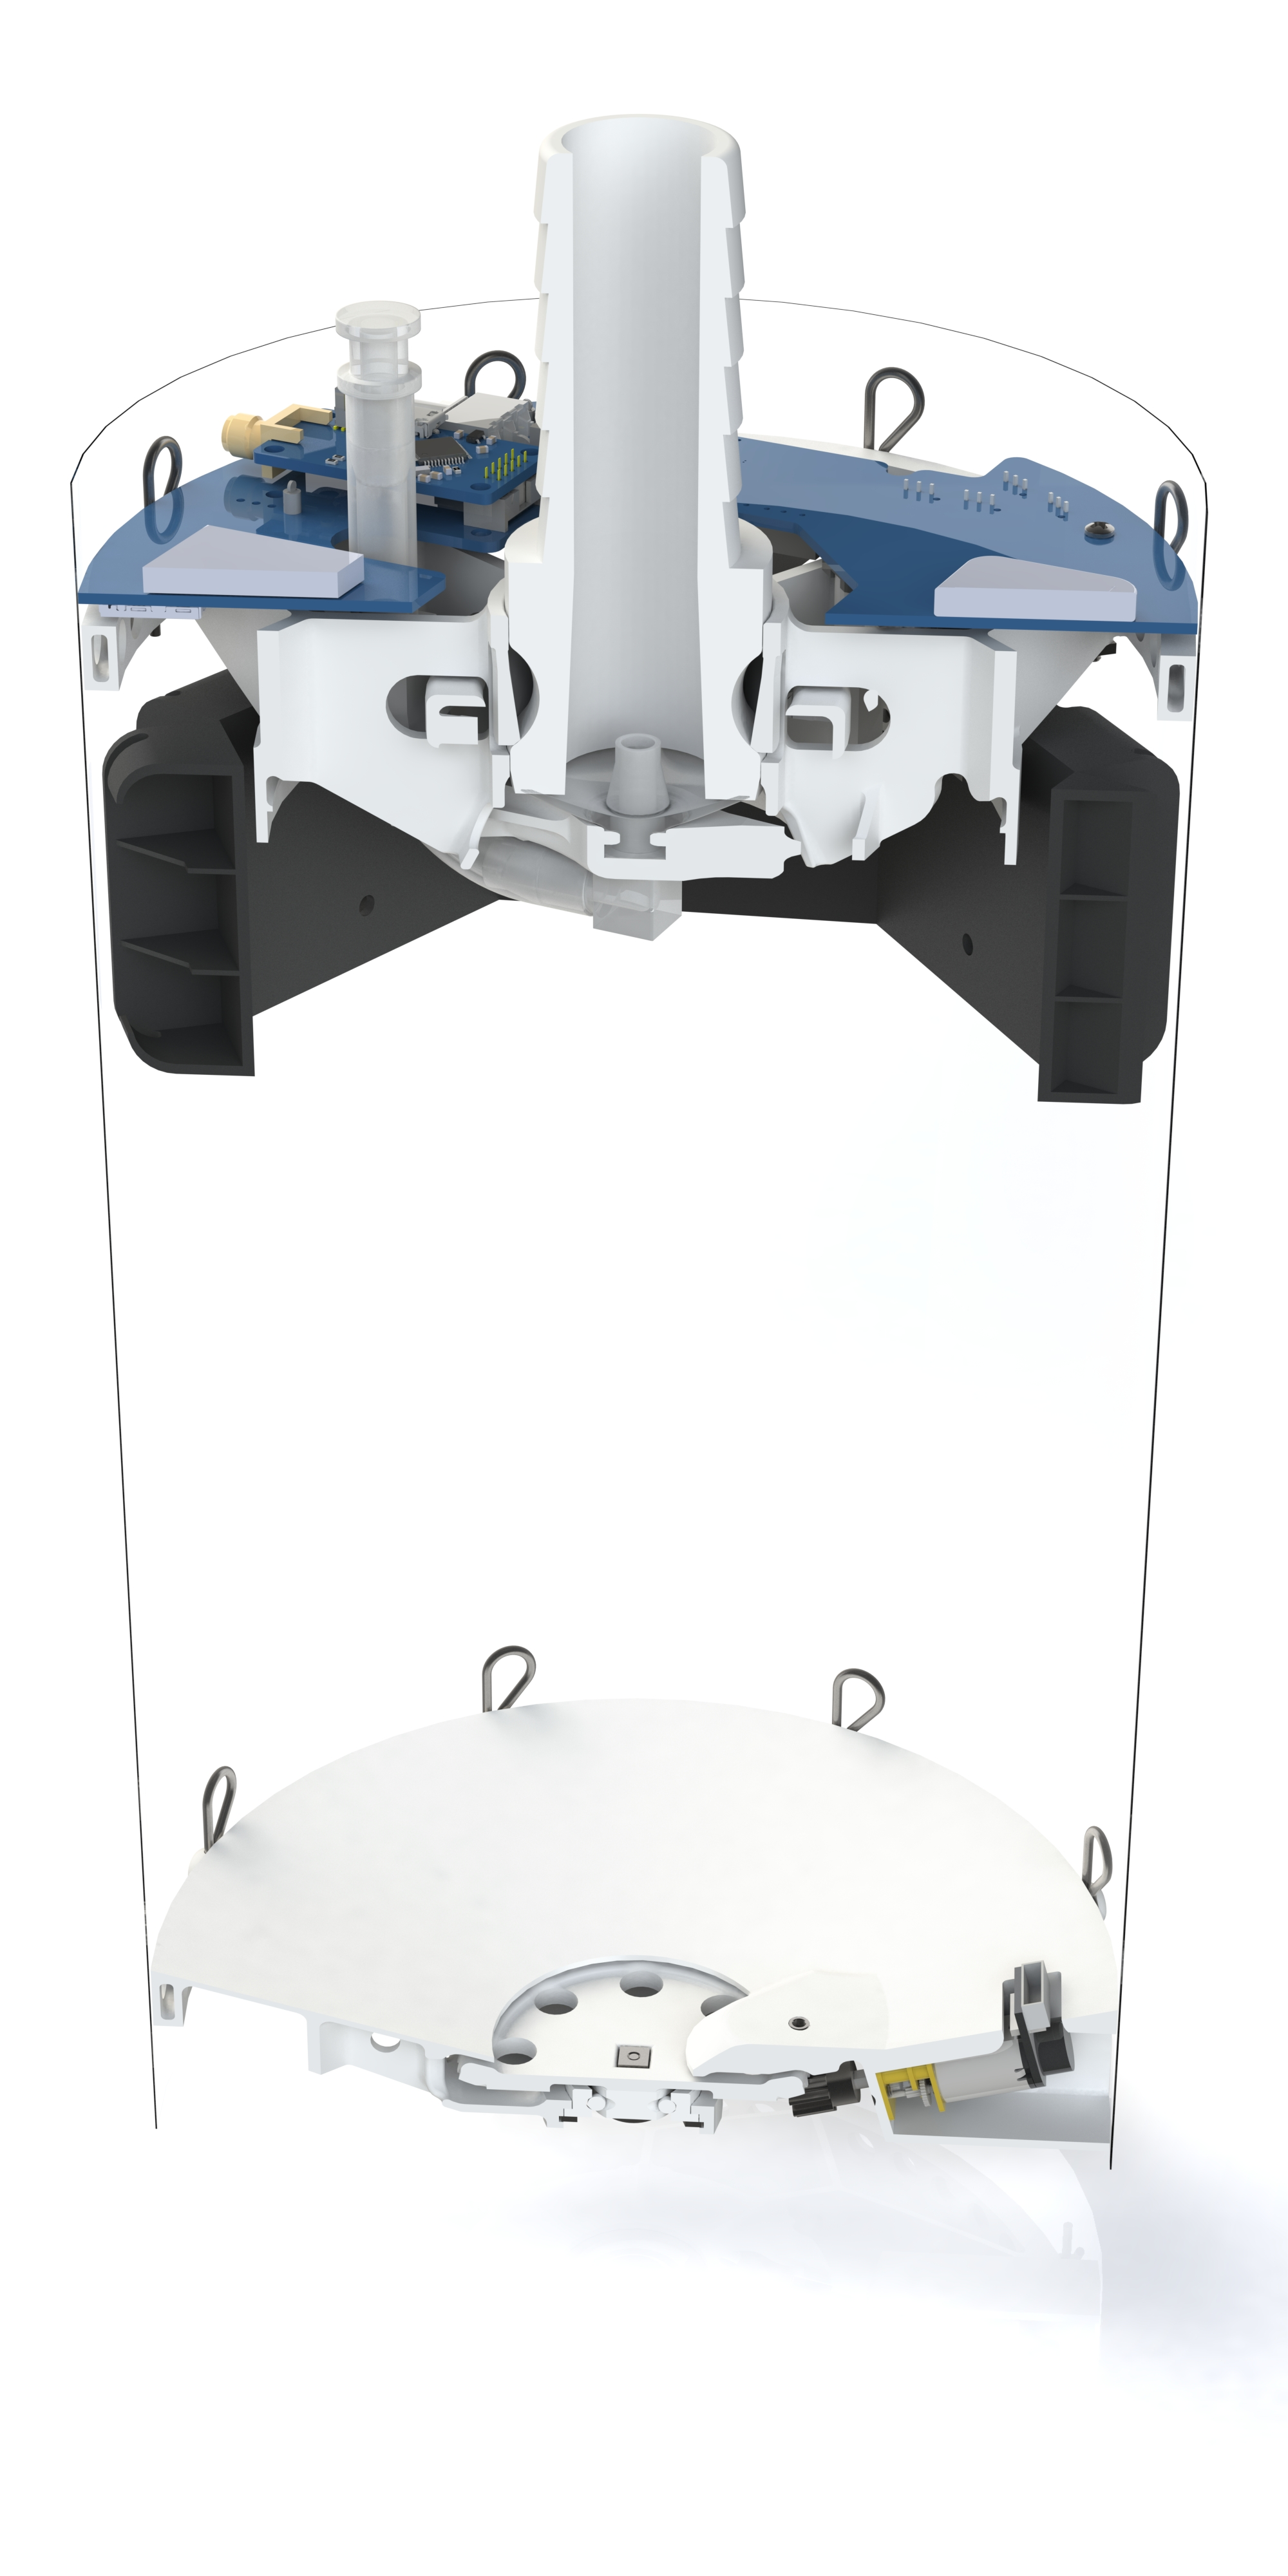
\includegraphics[width=0.4\linewidth,trim={0cm 13cm 0cm 5cm},clip]{render.jpg}\hspace{1cm}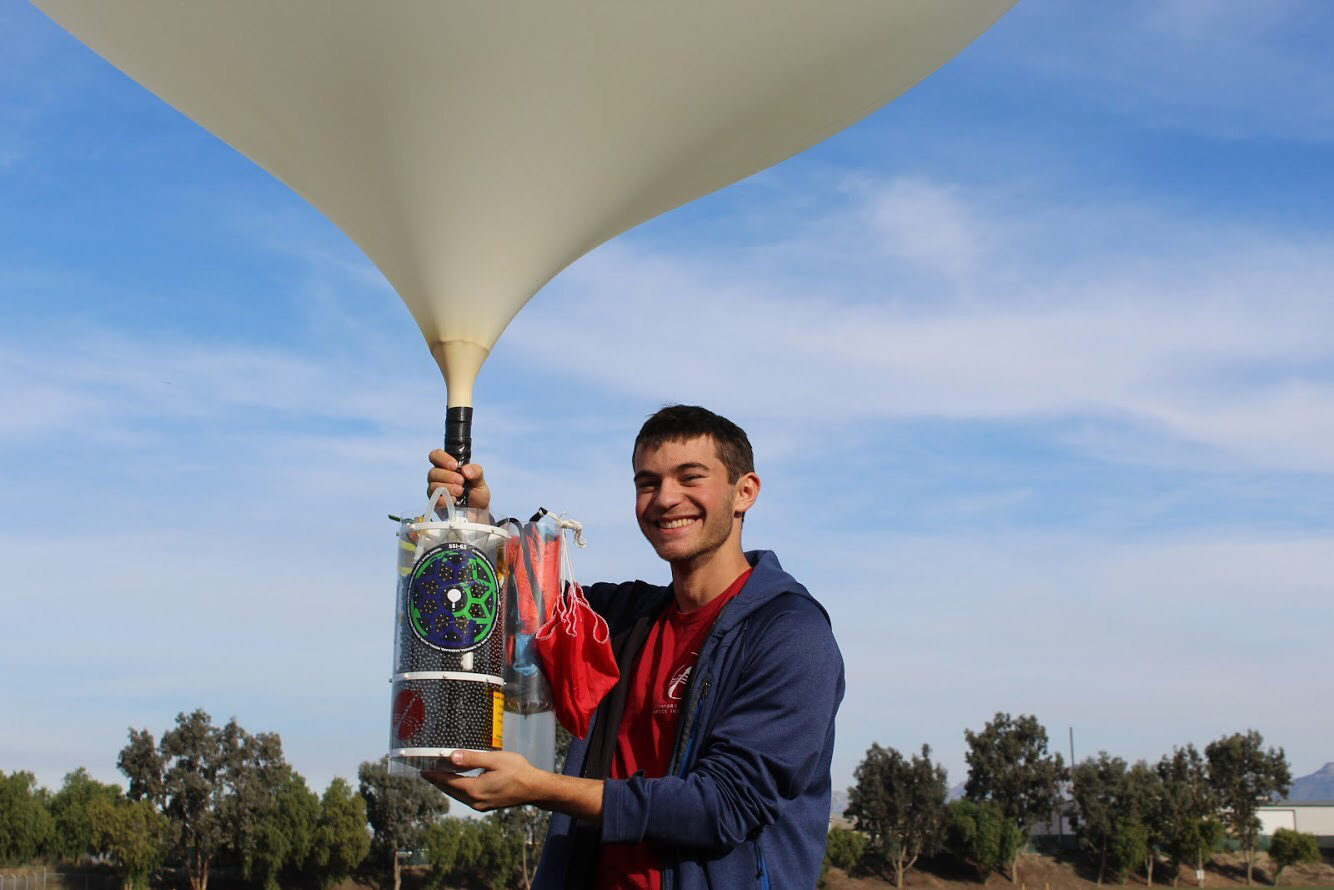
\includegraphics[width=0.4\linewidth,trim={12cm 2cm 25cm 12cm},clip]{vbpic.jpg}\end{center}
\end{frame}


\begin{frame}
\centering
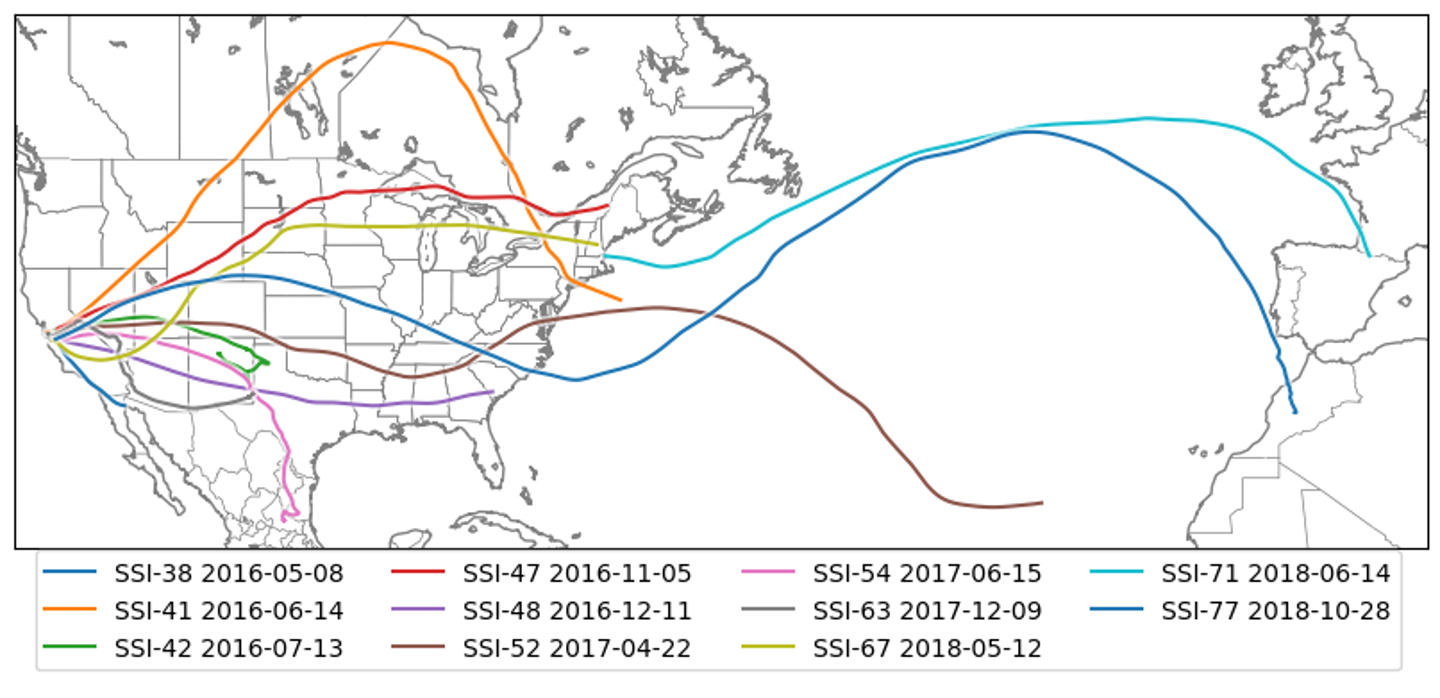
\includegraphics[width=0.9\linewidth]{valbal-map.png}
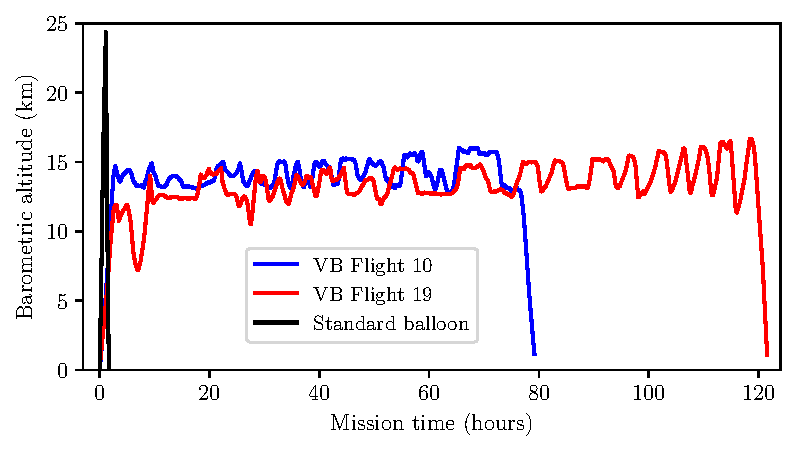
\includegraphics[width=0.6\linewidth]{thegraph.pdf}
%\vfill
\end{frame}

\section{Trajectory Planning}

\begin{frame}
\frametitle{Trajectory Planning}
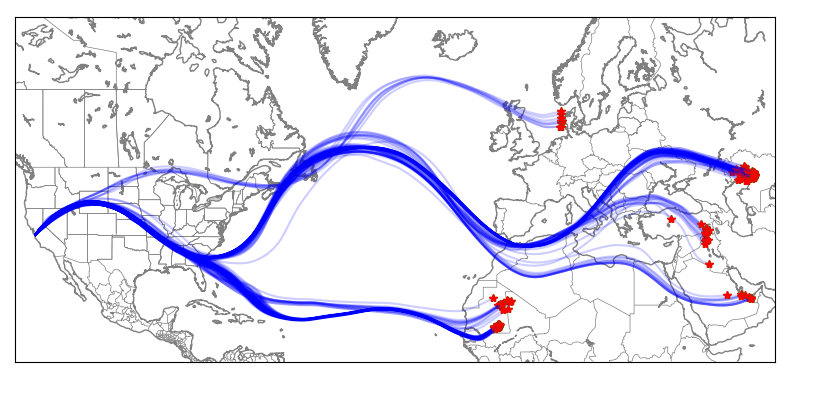
\includegraphics[width=\linewidth,trim={0cm 0cm .7cm 0cm},clip]{multitraj.png}
\end{frame}


\subsection{Background}

\begin{frame}
\frametitle{Tree search for station keeping}
\begin{itemize}
\item \citehere{DBorn}
\end{itemize}
\ig{0.9}{davis.png}
\end{frame}

\begin{frame}
\frametitle{MDP}
\begin{itemize}
\item \citehere{wolf2010}
\end{itemize}
\begin{columns}
\column{0.5\textwidth}
\ig{1}{blackmore1.png}
\column{0.5\textwidth}
\ig{1}{blackmore2.png}
\end{columns}
\end{frame}

\subsection{Formulation}

\begin{frame}
\frametitle{Formulation}
\begin{itemize}

\item System represented by states $s \in \mathcal{S}$
\item $\mathcal{S} = \mathcal{H} \times \Lambda \times \Phi \times \mathcal{T}$ (Time, Altitude, Longitude, Latitude)
\begin{itemize}
\item Physically intuitive to keep majority of state continuous---curse of dimensionality as we discretize.
\begin{itemize}
\item $h \in \mathcal{H}$: altitudes ($[0~\text{km},20~\text{km}]$)
\item $\lambda \in \Lambda$: longitudes ($[0, 2\pi]$)  
\item $\phi \in \Phi$: latitudes ($[-\pi/2,\pi/2]$)
\end{itemize}
\item $t \in \mathcal{T}$: time, defined in discrete steps of 10~min. Allows us to use simple Euler integration spatially to trace out wind field (altitude handled differently).
\end{itemize}
\item Atmospheric winds act on the balloon $w(h, \lambda, \phi, t) \to (u, v)$. $w$ given by \textsc{noaa} on 0.25\textdegree{} grid at various altitudes; interpolate in each variable.
\item Control policies $\theta(t) = (h_{\n{cmd}},e_{\n{tol}})$ command the altitude of the balloon and error tollerance around set altitude
\end{itemize}
\end{frame}

\begin{frame}
\frametitle{Formulation}
\begin{itemize}
\item Goal: formulate value function $V$ as a differentiable function of a (small) set of policy parameters $\theta$.
\begin{itemize}
\item Avoids having to discretize a huge state space as in most MDP formulations.
\end{itemize}
\item Optimize $V$ via a gradient method, \eg\, $\theta^{k+1} = \theta^k + \alpha_k \nabla_\theta V(\theta)$. for stepsize $a_k$
\item Allows us to preserve key properties of the spaces we're in:
\begin{itemize}
\item We preserve smoothness of the value function: the wind field is not random, and has a rather small spatial frequency.
\item We preserve the continuity of our variables: altitude, latitude, longitude need small discretization to be realistic.
\item We will be able to handle stochasticity without blowing up the size of the problem.
\end{itemize}
\end{itemize}
\end{frame}


\begin{frame}
\frametitle{Formulation: example}
\begin{itemize}
\item Suppose we want to maximize longitudinal distance of final point after $N$ steps (say $N=720$, 5 days).
\item Final longitude is the result of doing a simulation rollout, using Euler integration in latitude and longitude.
\item $V = \lambda_f=\lambda_0 + v_1(t_1, h_1,\phi_1,\lambda_1)\Delta t + \cdots + v_N(t_N, h_N, \phi_N,\lambda_N)\Delta t$.


\item Need to parametrize $V$. We control altitude of the balloon (see later). Simplest formulation: define waypoints $\theta_1,\dots,\theta_k$ at points $T_1,\dots,T_k$, and assume balloon goes linearly between waypoints: $h_i=\theta_j + (t_i-T_j)\frac{\theta_{j+1}-\theta_j}{T_{j+1}-T_j}$. Ability to do stochastic formulations (later).
%\item However each velocity depends on altitude, which means that each successive longitude depends on all previous altitudes\dots OH GOD THE BLOCK IS REAL
\end{itemize}
\end{frame}

\begin{frame}
\begin{align*}
h(t) &= \begin{cases}
\theta_1 + (t-t_1)\frac{\theta_2-\theta_1}{t_2-t_1} \qquad & t_1 \leq t < t_2\\
\cdots\\
\theta_{n-1} + (t-t_{n-1})\frac{\theta_n-\theta_{n-1}}{t_n-t_{n-1}} \qquad & t_{n-1} \leq t < t_n
\end{cases}\\
w_{\{\lambda,\phi\}}(\lambda,\phi,h,t) &= \text{bilinear interpolation in $(\lambda,\phi)$, linear in $t,h$ from \textsc{NOAA}}
\end{align*}
\begin{align*}
&(h_0, t_0, \phi_0, \lambda_0)\\
&\begin{cases}
h_1 = h(t_1)\\
\lambda_1 = \lambda_0 + \Delta t \cdot w_\lambda(\lambda_0, \phi_0, h_0, t_0)\\
\phi_1 = \phi_0 + \Delta t \cdot w_\phi(\lambda_0, \phi_0, h_0, t_0)
\end{cases}\\
&\begin{cases}
h_2 &= h(t_2)\\
\lambda_2 &= \lambda_1 + \Delta t \cdot w_\lambda(\lambda_1, \phi_1, h_1, t_1)\\
&{\scriptstyle =\lambda_0 + \Delta t \cdot w_\lambda(\lambda_0, \phi_0, h_0, t_0)} \\[-0.2cm]
&{\scriptstyle \qquad + w_\lambda(\lambda_0 + w_\lambda(\lambda_0, \phi_0, h_0, t_0) \Delta t, \phi_0 +  w_\phi(\lambda_0, \phi_0, h_0, t_0)\Delta t, h_(t_1), t_1)\Delta t} 
\end{cases}\\
&\cdots\\
&\frac{\partial \lambda_n}{\partial \theta_i}\neq 0\text{, follow the computation graph to compute derivative}
\end{align*}

%\[s_{k+1} = a(s_k,\theta(t_k))\]
%\[s_{k+1} = a(\dots a(a(s_0,\theta(t_0)),\theta(t_1))\dots )\theta(t_k))\]
%\[\frac{d s_{k+1}}{d\theta(t_k)} = a(\dots a(a(s_0,\theta(t_0)),\theta(t_1))\dots ),\theta(t_k))\]
\end{frame}

\begin{frame}
\frametitle{Stochastic formulation}
\begin{itemize}
\item Previous formulation does not account for noise---balloon can't hit linearly interpolated altitude waypoints exactly! (Not without wasting tonnes of ballast, anyway.)
\item Onboard control algorithm has two parameters: $h_\text{cmd}$ (setpoint) and $e_\text{tol}$ (tolerance). Approximate balloon as being somewhere in $h_\text{cmd}\pm e_\text{tol}$ randomly.
\item However, position within the tolerance is correlated between timesteps.
\begin{itemize}
\item If balloon was at $h_\text{cmd} - 0.98e_\text{tol}$ at $t=0$, it's unlikely to be at $h_\text{cmd} + 0.5e_\text{tol}$ at $t=10~\text{min}$.
\end{itemize}
\item Solution: parametrize in terms of a slow-moving random walk $\lambda(t)$.
\end{itemize}
\end{frame}

\begin{frame}
\frametitle{Stochastic formulation}

\begin{itemize}
\item Refined differentiable altitude:
\[h(t; \lambda) =
\text{LinInterp}\left(t, t_i \to h_{\text{cmd},i} + \lambda(t_i) e_{\text{tol},i}\right)
\]
where $-1 \leq \lambda(t) \leq 1$ is sampled from realistic balloon trajectories (e.g. stochastic altitude controller simulations).
\item Note we introduced randomness into the simulation without blowing up the size of the state space!
\item If we let $\lambda(t)=0$, we recover certainty equivalent formulation above.
\item If we sample multiple random $\lambda(t)$, we can build a stochastic value function:
\[\tilde V = \sum_{\text{random}~\lambda}^K V(t_f; \lambda)\]
\item If we increase $K$ we capture the variance distribution with more fidelity.
\end{itemize}

\end{frame}

\begin{frame}
\frametitle{algorithm}
\begin{algorithmic}[1]
\Procedure{StocasticMPC}{$S_1,S_2$}
\State$s:$ intial sim state
\While{not converged}
\State$obj:$ objective object
\For{$i \in \{0, 1, \dots, N-1\}$}
\State Sim : simulation object
\EndFor 

check convergence
\EndWhile
\EndProcedure
\end{algorithmic}
\end{frame}

\subsection{Results}

\begin{frame}
\frametitle{Certainty Equivalent}
\begin{columns}
\column{0.6\linewidth}
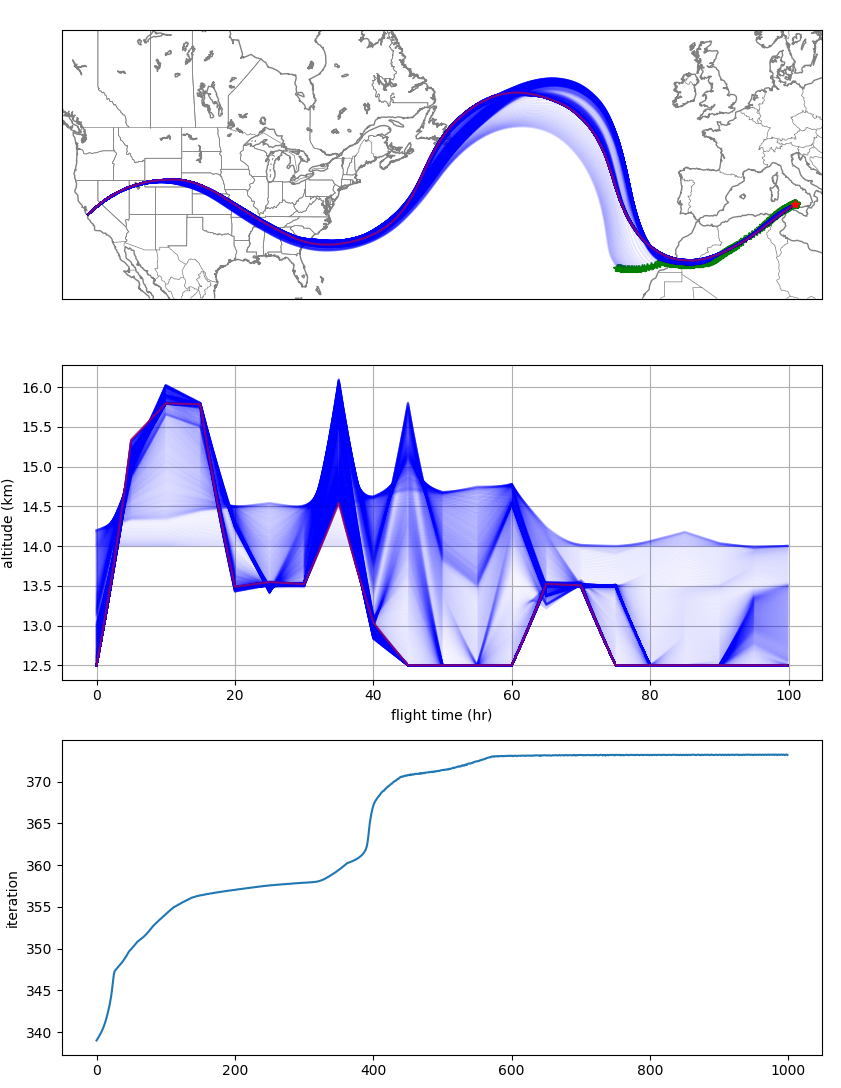
\includegraphics[width=1\linewidth,trim={0 9.5cm 0 0cm},clip]{certaintyeq.png}
\column{0.5\linewidth}
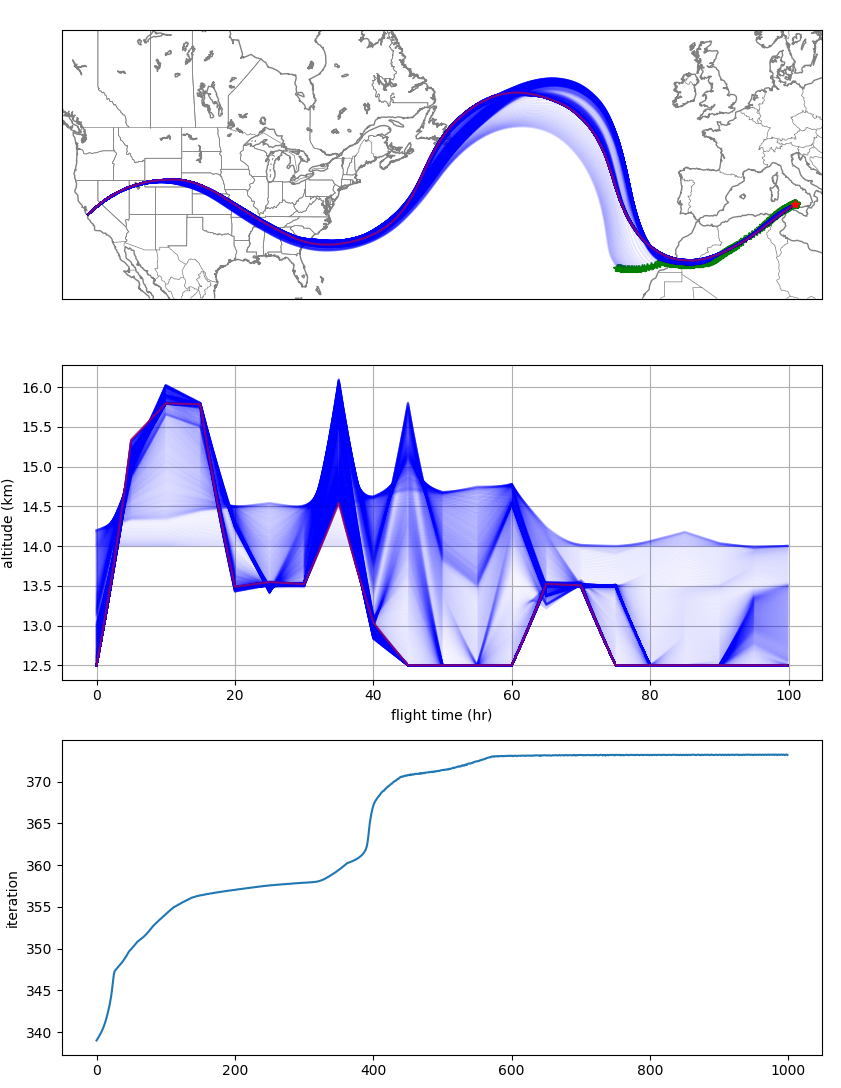
\includegraphics[width=1\linewidth,trim={0 0cm 0 18.3cm},clip]{certaintyeq.png}
\end{columns}
\end{frame}

\begin{frame}
\frametitle{Stocasstic}
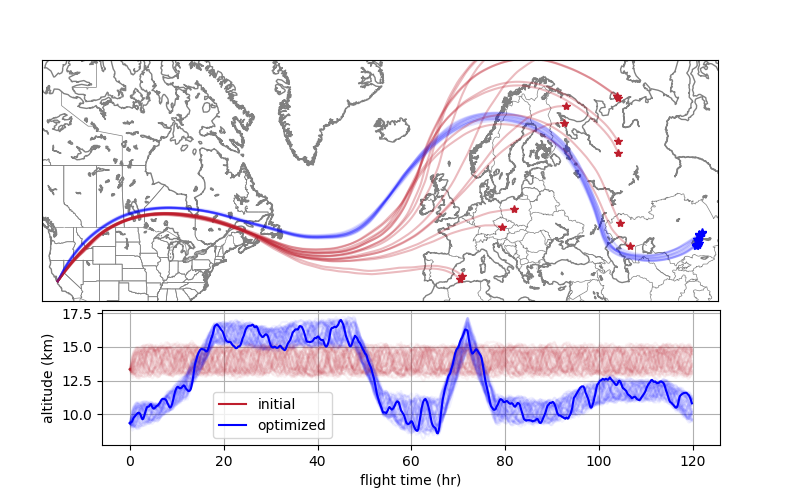
\includegraphics[width=1\linewidth,trim={0 0cm 0 0cm},clip]{datasheetfig.png}
\end{frame}

\subsection{Flight Test}

\begin{frame}
\frametitle{Valbal Flights}
\ig{1}{valbal-map.png}
\end{frame}

\begin{frame}
\frametitle{SSI-77 Launch (Oct 28)}
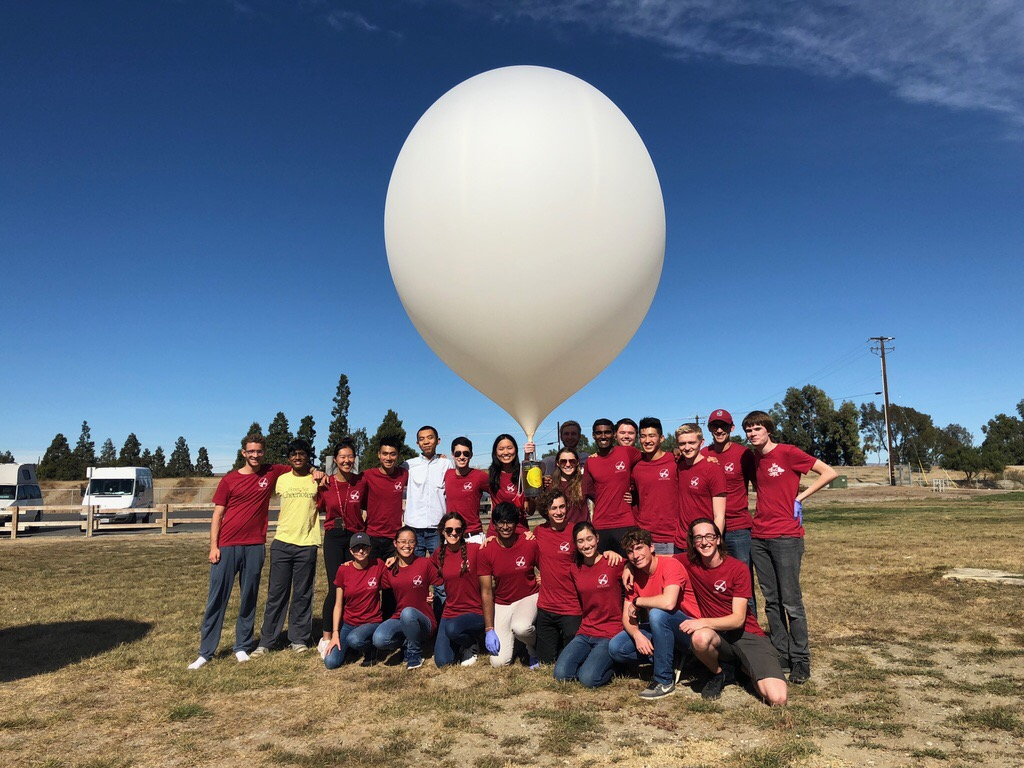
\includegraphics[width=1\linewidth,trim={0 2cm 0 2cm},clip]{launch.jpg}
\end{frame}

\begin{frame}
\frametitle{Mission Control}
\hspace*{-1cm}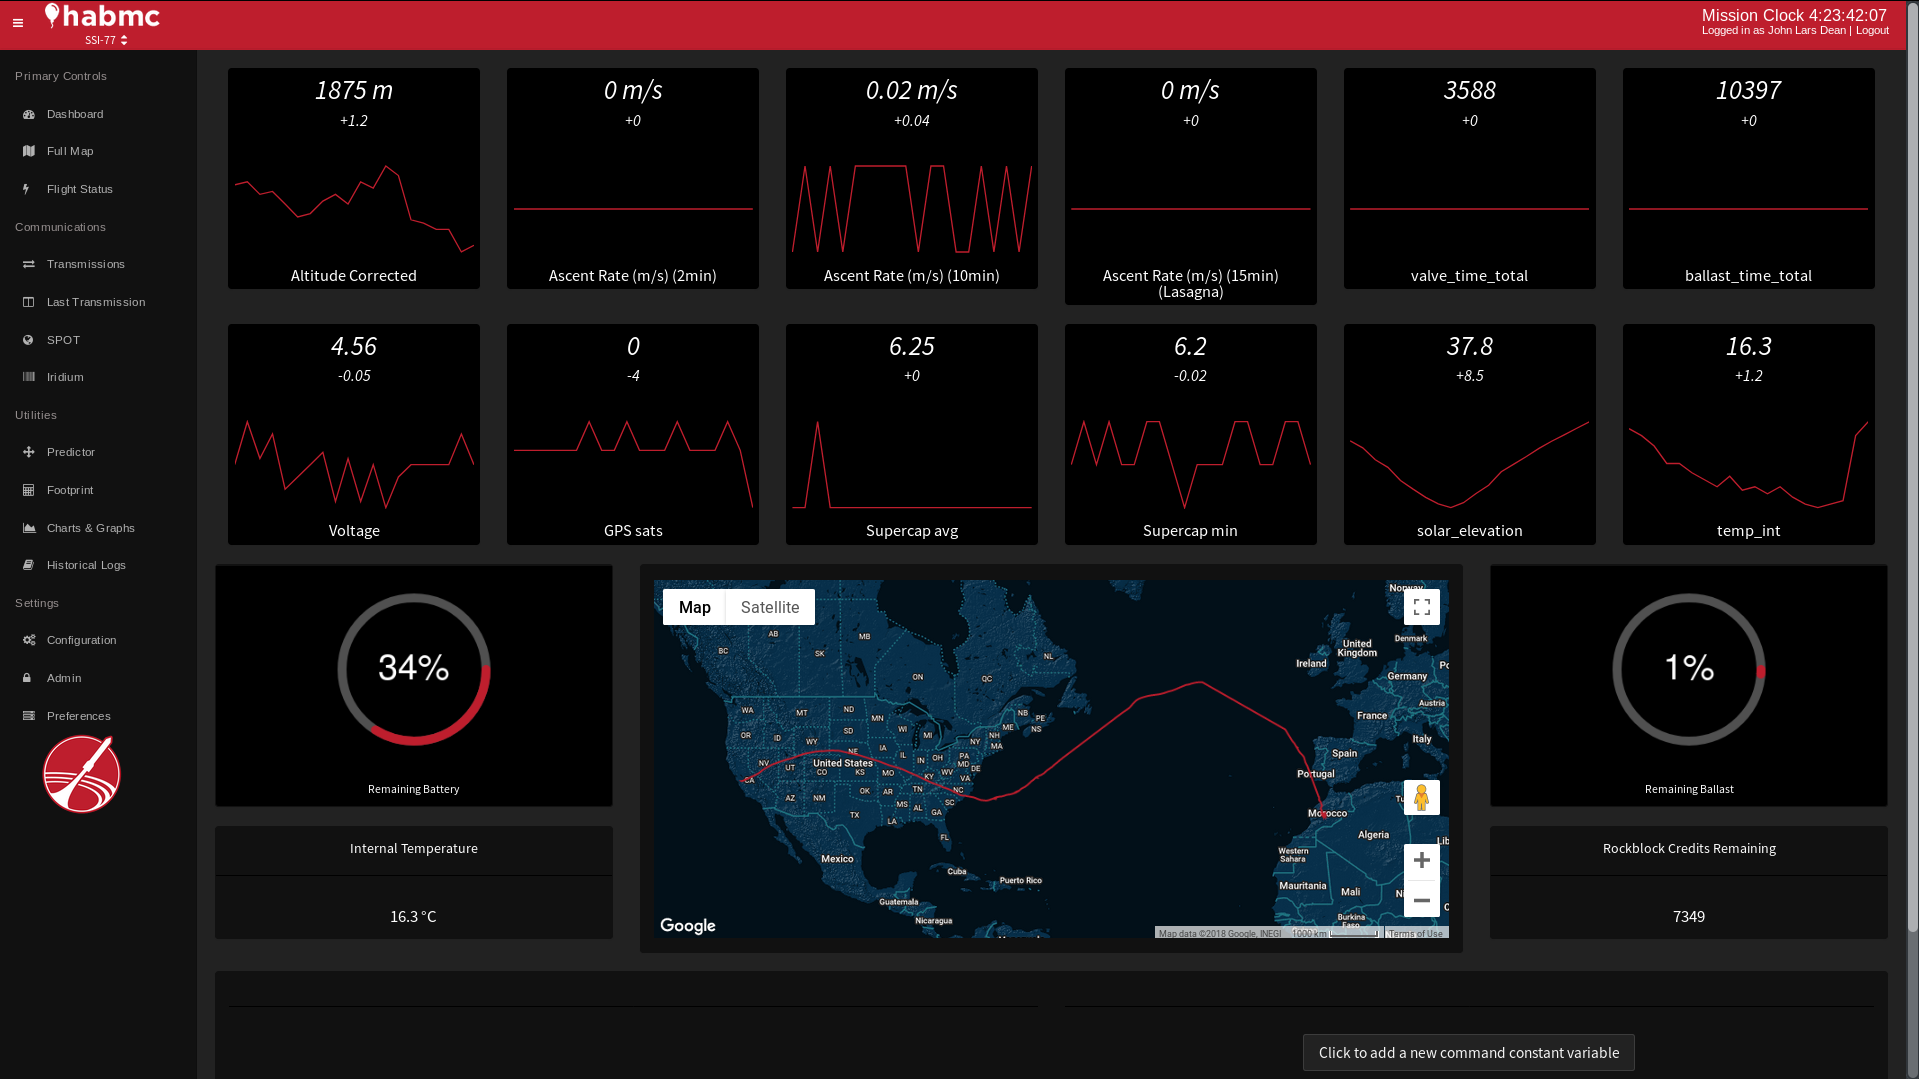
\includegraphics[width=1.2\linewidth,trim={0 0cm 0 0cm},clip]{habmc.png}
\end{frame}

\begin{frame}
\frametitle{Flight Optimization}
\begin{center}
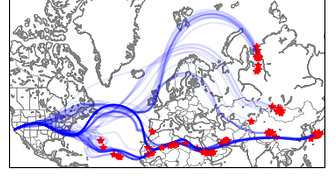
\includegraphics[width=1\linewidth,trim={0 0cm 0 0cm},clip]{f1.png}
\end{center}
\end{frame}
\begin{frame}
\frametitle{Flight Optimization}
\begin{center}
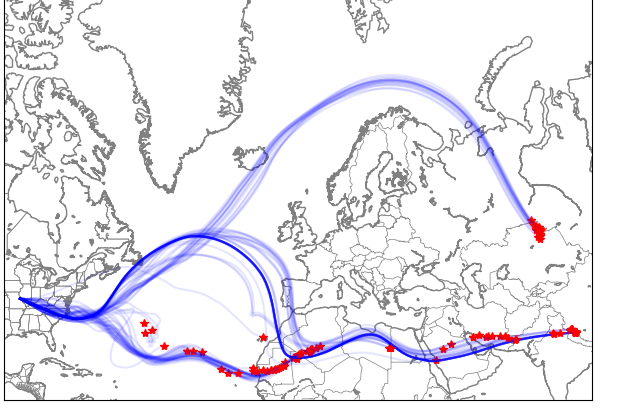
\includegraphics[width=1\linewidth,trim={0 0cm 0 0cm},clip]{f2.png}
\end{center}
\end{frame}
\begin{frame}
\frametitle{Flight Optimization}
\begin{center}
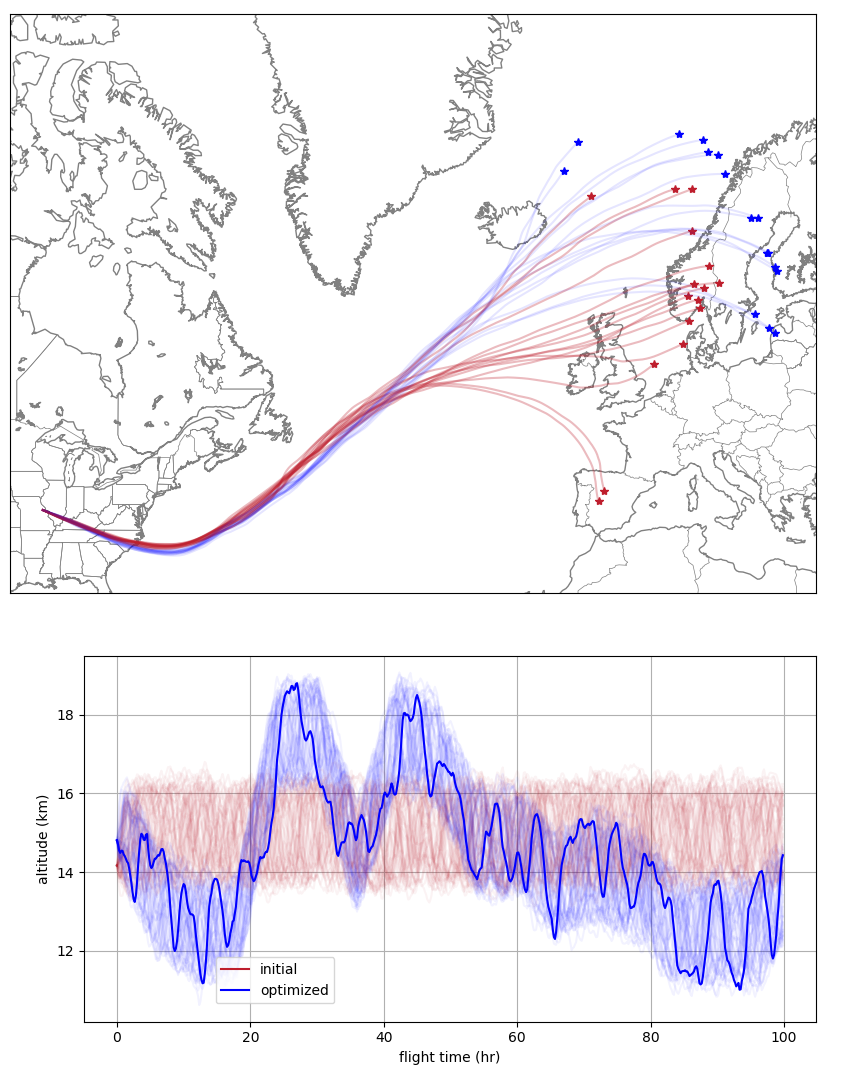
\includegraphics[width=.6\linewidth,trim={0 0cm 0 0cm},clip]{f3.png}
\end{center}
\end{frame}
\begin{frame}
\frametitle{Flight Optimization}
\begin{center}
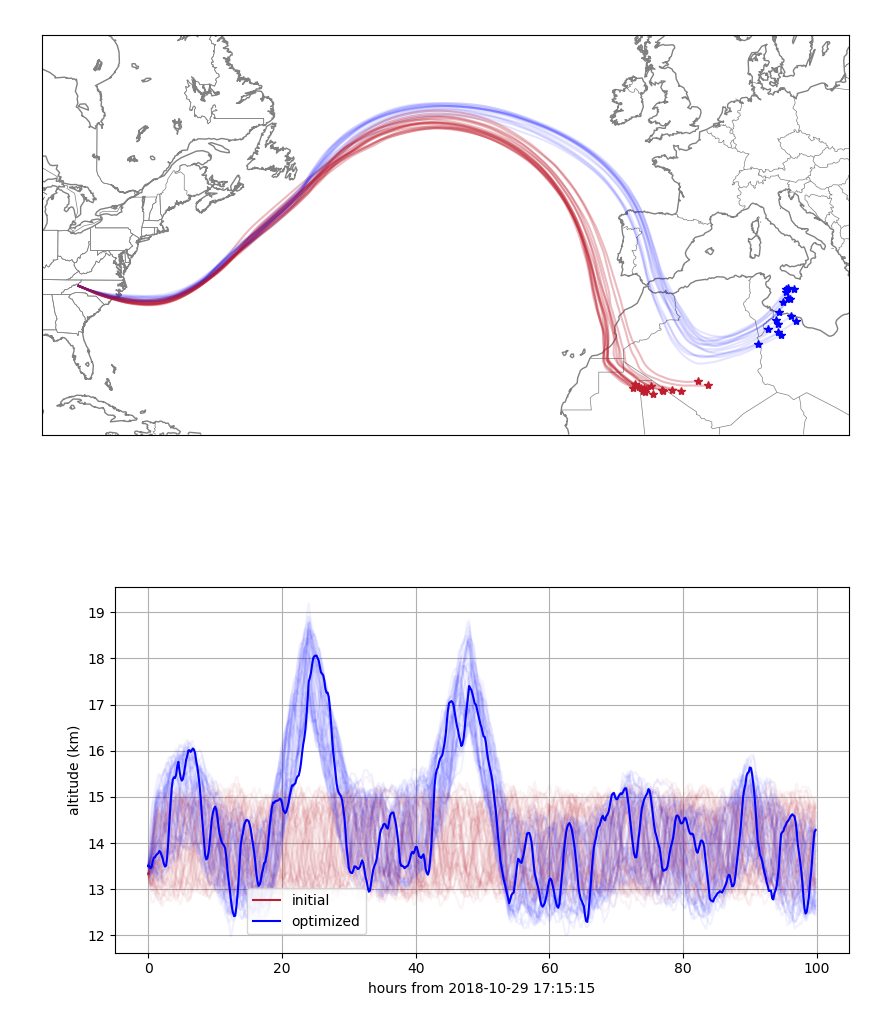
\includegraphics[width=.6\linewidth,trim={0 0cm 0 0cm},clip]{f4.png}
\end{center}
\end{frame}
\begin{frame}
\frametitle{Flight Optimization}
\begin{center}
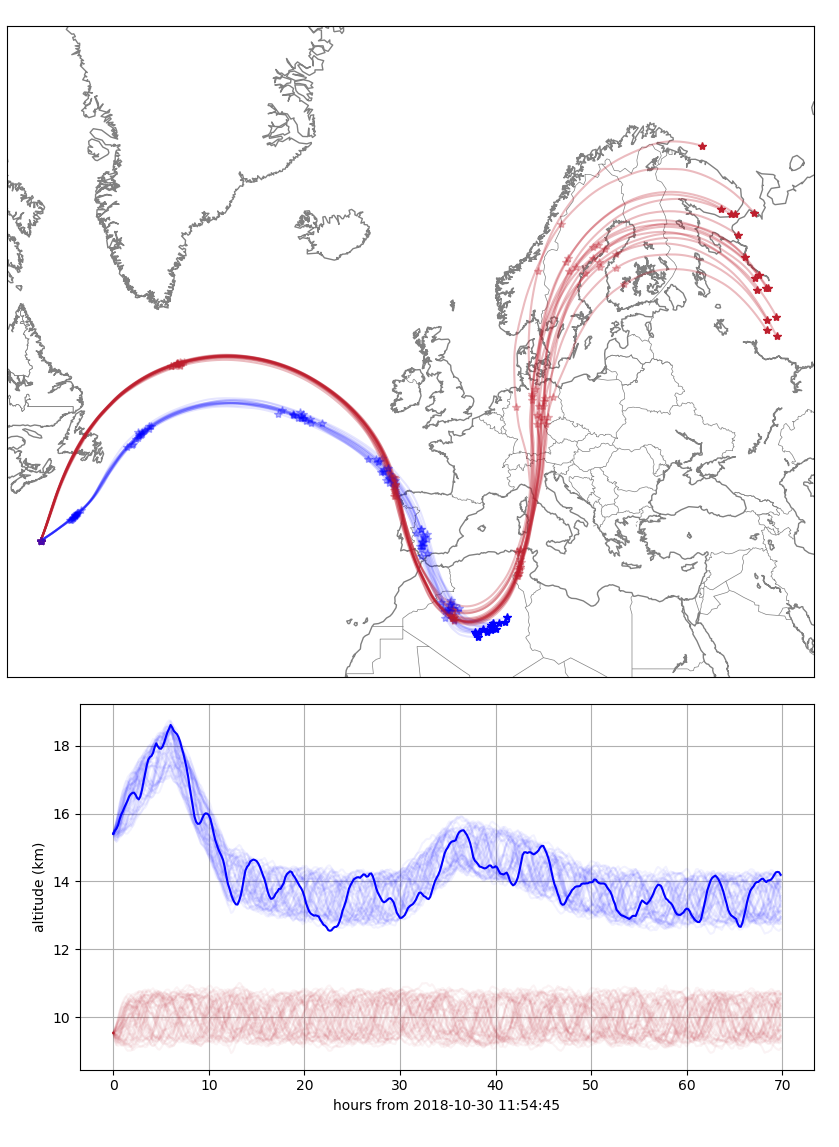
\includegraphics[width=.6\linewidth,trim={0 0cm 0 0cm},clip]{f5.png}
\end{center}
\end{frame}
\begin{frame}
\frametitle{Flight Optimization}
\begin{center}
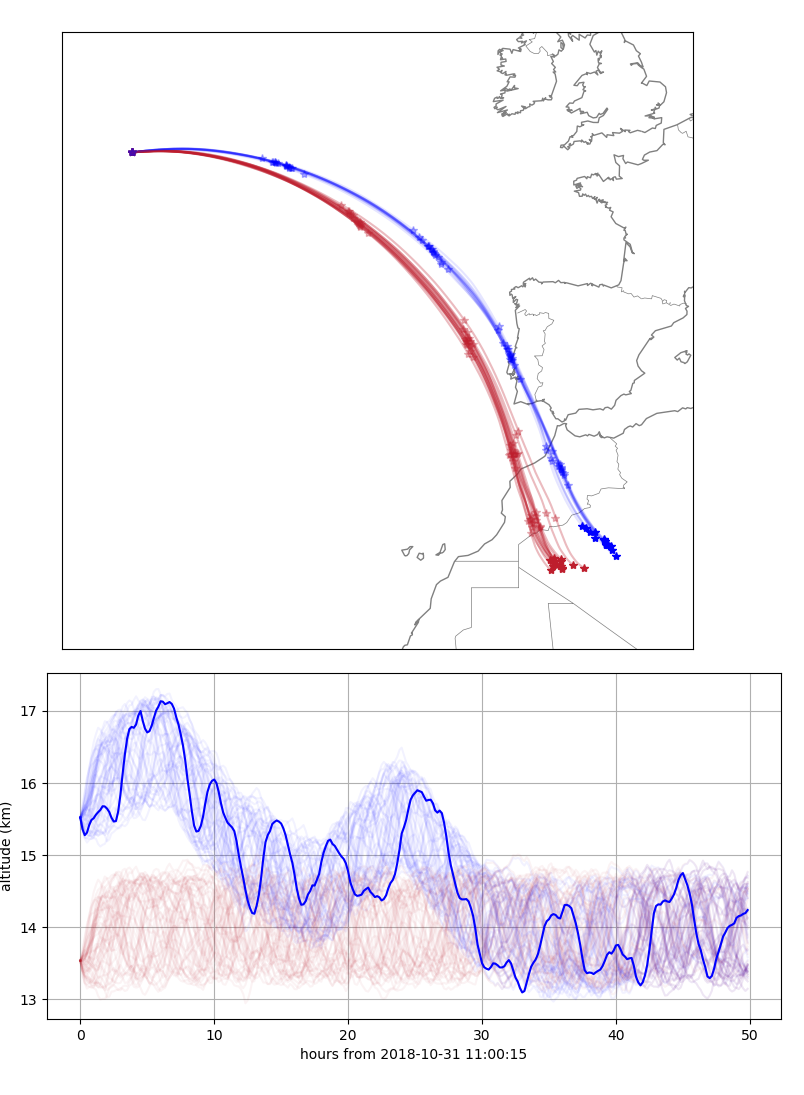
\includegraphics[width=.6\linewidth,trim={0 0cm 0 0cm},clip]{f6.png}
\end{center}
\end{frame}
\begin{frame}
\frametitle{Flight Optimization}
\begin{center}
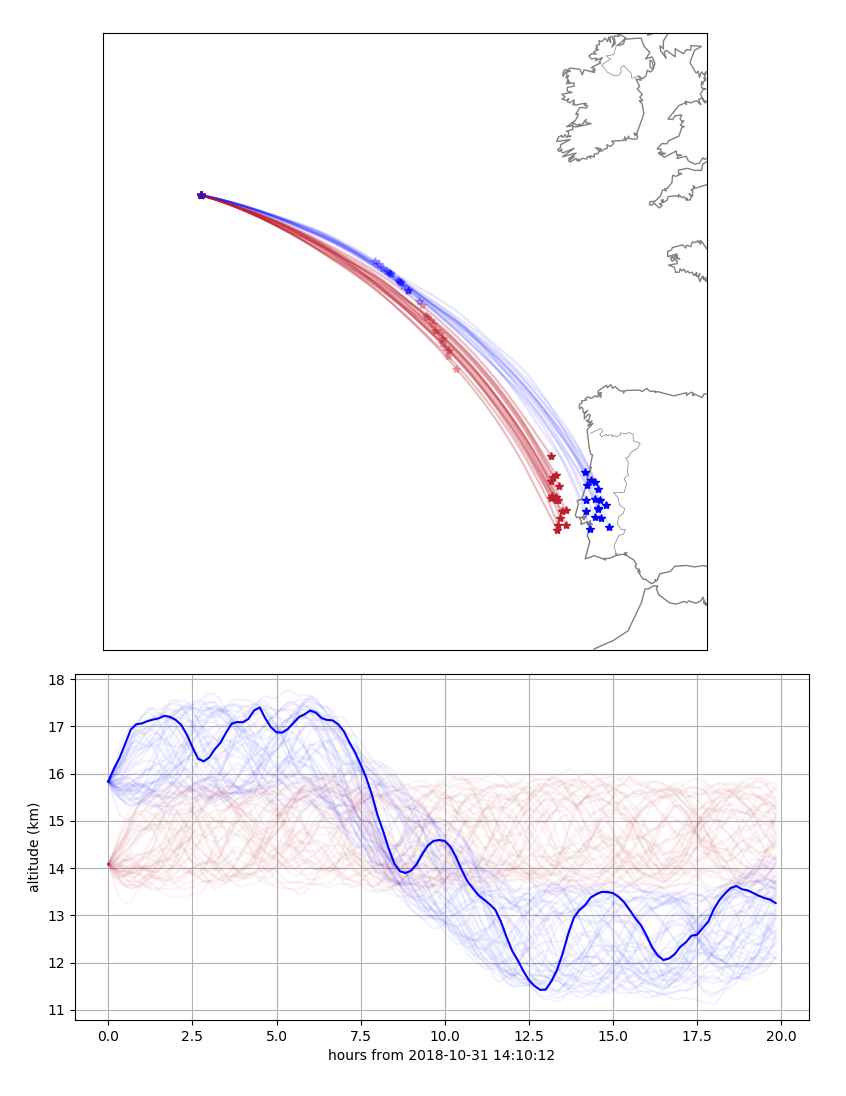
\includegraphics[width=.6\linewidth,trim={0 0cm 0 0cm},clip]{f7.png}
\end{center}
\end{frame}
\begin{frame}
\frametitle{Flight Optimization}
\begin{center}
\hspace*{-1.4cm}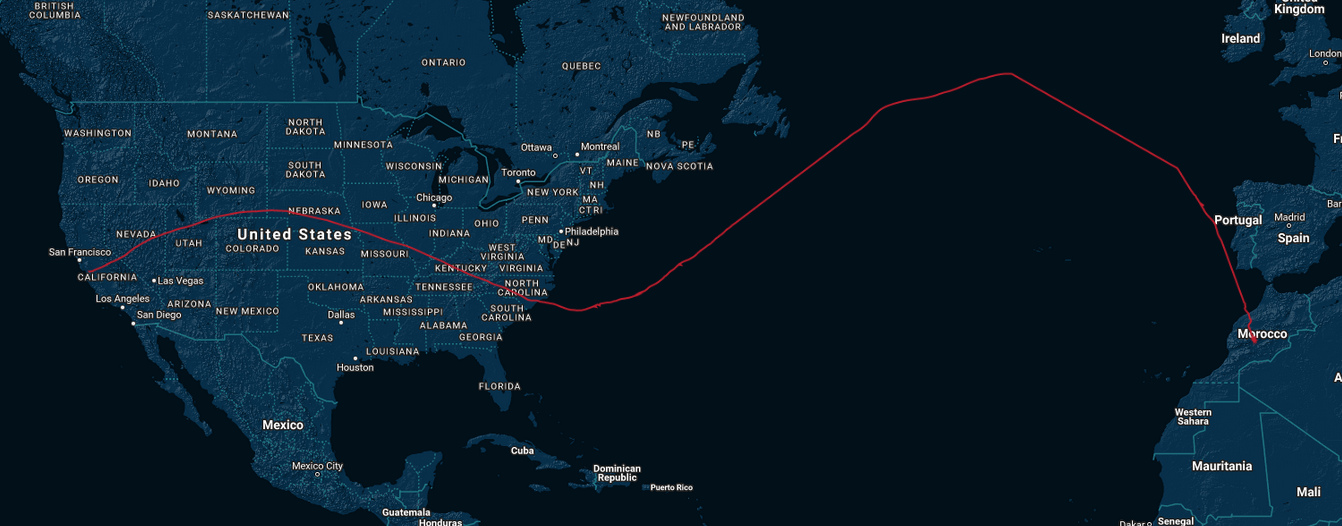
\includegraphics[width=1.2\linewidth,trim={0 0cm 0 0cm},clip]{f8.png}
\end{center}
\end{frame}

\subsection{Architecture}
\begin{frame}{Architecture}
\end{frame}

\section{Altitude Control}
\subsection{System Dynamics}

\begin{frame}
\frametitle{System Dynamics}
\begin{columns}
\column{0.6\textwidth}
\begin{itemize}\itemsep=12pt
\item Assumptions
\vspace*{0.5em}
\begin{itemize}
\item $F_d \propto v$ i.e. drag is linear.
\item $F_l - F_g = F_d$ i.e. the balloon is always at terminal velocity 
\end{itemize}
\item Equations of motion
\vspace*{0.5em}
\begin{itemize}
\item let $\ell = F_{\ell} - F_g$ be the net lift on the balloon
\item $\dot \ell$ is commanded by controller
\item $\dot v(t) = k_d (\dot \ell(t) + w_{\dot \ell} (t))$
\item $\dot h(t) = v(t) +  w_v(t)$
\item $\mathcal{L}\{h(t) / \dot \ell (t) \} = k_{d} / s^2$
\end{itemize}
\end{itemize}

\column{0.4\textwidth}

\begin{center}
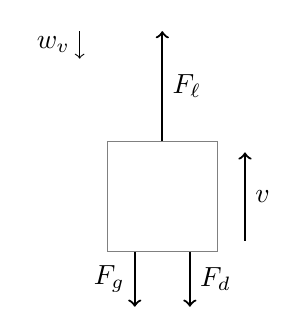
\begin{tikzpicture}[scale=0.7]
    \draw[gray] (-1,-1) rectangle (1,1);
    \draw[thick,->] (0,1) -- (0,3) node[midway,right]{$F_{\ell}$};
    \draw[thick,->] (.5,-1) -- (.5,-2) node[midway,right]{$F_d$};
    \draw[thick,->] (-.5,-1) -- (-.5,-2) node[midway,left]{$F_g$};
    \draw[thick,->] (1.5,-0.8) -- (1.5,0.8) node[midway,right]{$v$};
    \draw[->] (-1.5,3) -- (-1.5,2.5) node[midway,left]{$w_v$};
\end{tikzpicture}
\end{center}
$F_d$: Force of drag\\
$F_g$: Gravity\\
$F_{\ell}$: Buoyant force\\
$v$: vertical velocity of balloon\\
$w_v$: vertical velocity of surrounding air
\end{columns}
\end{frame}

\begin{frame}
\frametitle{Plant Block Diagram}
\begin{center}
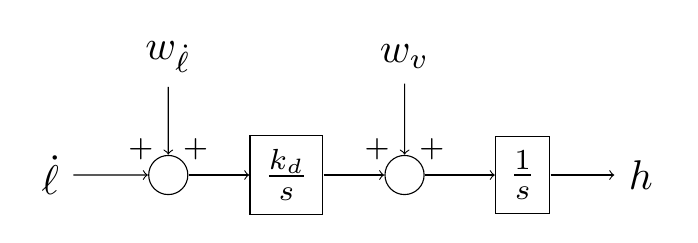
\begin{tikzpicture}[scale=2,
     block/.style = {draw, rectangle,node distance=1cm},
     input/.style = {node distance=1cm},
     output/.style = {node distance=1cm},
     arrow/.style={draw, -latex,node distance=2cm},
     pinstyle/.style = {pin edge={latex-, black,node distance=2cm}},
     sum/.style = {draw, circle, node distance=1cm},
     gain/.style = {regular polygon, regular polygon sides=3,draw, fill=white, text width=1em,
      inner sep=0mm, outer sep=0mm,
      shape border rotate=-90}
    ]
    \begin{scope}[scale=.75, transform shape]
    \node [input] (cinput) {$\dot \ell$};
    \node [sum, right of=cinput] (dlift) {};
    \node [input, above of=dlift] (ldist) {$w_{\dot \ell}$};
    \node [block, right of=dlift] (lint) {$\frac{k_d}{s}$};
    \node [sum, right of=lint] (velocity) {};
    \node [input, above of=velocity] (vdist) {$w_v$};
    \node [block, right of=velocity] (vint) {$\frac{1}{s}$};
    \node [output, right of=vint] (h) {$h$};

    \draw[->] (cinput) -- (dlift) node [above left] {\scriptsize +};
    \draw[->] (ldist) -- (dlift) node [above right] {\scriptsize +};
    \draw[->] (dlift) -- (lint);
    \draw[->] (lint) -- (velocity) node [above left] {\scriptsize +};
    \draw[->] (vdist) -- (velocity) node [above right] {\scriptsize +};
    \draw[->] (velocity) -- (vint) node [above right] {};
    \draw[->] (vint) -- (h) node [above right] {};
    \end{scope}
\end{tikzpicture}
\end{center}
\vspace{0cm}
$\dot \ell$: commanded change in lift (valve and ballast actions) \\
$w_{\dot \ell}$: atmospheric lift disturbance \\
$w_v$: atmosphereic velocity disturbance \\
$h$: altitude 
\[x = \mx{c}{h \\ v} \qquad u = \dot \ell\]
\[\dot x = \mx{cc}{0 & 1 \\ 0 & 0}x + \mx{cc}{0 \\ k_d} u + \mx{c}{w_v \\ k_d w_{\dot \ell}}\]

\end{frame}

\begin{frame}
\frametitle{Controller Block Diagram}
\resizebox{11cm}{!}{
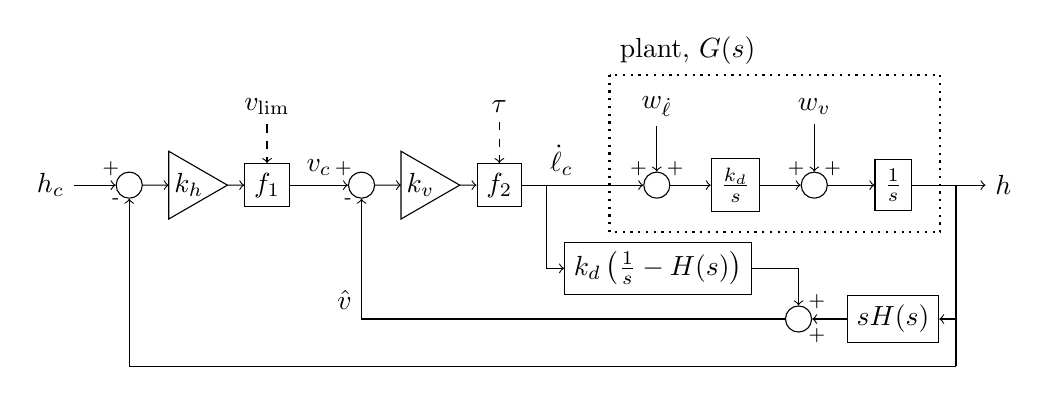
\begin{tikzpicture}[scale=2,
     block/.style = {draw, rectangle,node distance=1cm},
     input/.style = {node distance=1cm},
     output/.style = {node distance=1cm},
     arrow/.style={draw, -latex,node distance=2cm},
     pinstyle/.style = {pin edge={latex-, black,node distance=2cm}},
     sum/.style = {draw, circle, node distance=1cm},
     gain/.style = {regular polygon, regular polygon sides=3,draw, fill=white, text width=1em,
      inner sep=0mm, outer sep=0mm,
      shape border rotate=-90}
    ]
        
    \node [input] (hcmd) {$h_c$};
    \node [sum,right of=hcmd] (hsum) {};    
    \node [gain,right of=hsum, node distance=0.75cm] (K1) {$k_h$};
    \node [block, right of=K1] (N1) {$f_1$};
    \node [sum,right of=N1, node distance=1.2cm] (vsum) {};
    \node [input,above of=N1] (vlim) {$v_{\mathrm{lim}}$};
    \node [gain, right of=vsum,node distance=0.75cm] (K2) {$k_v$};
    \node [block, right of=K2] (N2) {$f_2$};
    \node [sum, right of=N2, node distance=2cm] (dlift) {};
    \node [input,above of=N2] (etol) {$\tau$};
    \node [input, above of=dlift] (ldist) {$w_{\dot \ell}$};
    \node [block, right of=dlift] (lint) {$\frac{k_d}{s}$};
    \node [sum, right of=lint] (velocity) {};
    \node [input, above of=velocity] (vdist) {$w_v$};
    \node [block, right of=velocity] (vint) {$\frac{1}{s}$};
    \node [output, right of=vint,node distance=1.4cm] (h) {$h$};
    \node [block, below of=vint,node distance=1.7cm] (H1) {$sH(s)$};
    \node [block, below right = .6 cm and -1.3 cm of dlift] (H2) {$k_d\left(\frac{1}{s}-H(s)\right)$};
    \node [sum, left of=H1,node distance=1.2cm] (fsum) {};

    \draw[->] (hcmd) -- (hsum) node [above left] {\scriptsize +};
    \draw[->] (hsum) -- (K1);
    \draw[->] (K1) -- (N1);
    \draw[->] (N1) -- node [above] {$v_c$} (vsum) node [above left] {\scriptsize +};
    \draw[->] (vsum) -- (K2);
    \draw[->] (K2) -- (N2);
    \draw[->,dashed] (etol) -- (N2);
    \draw[->,dashed] (vlim) -- (N1);
    \draw[->] (N2) -- node [above left] {$\dot \ell_c$} (dlift)  node [above left] {\scriptsize +};
    \draw[->] (ldist) -- (dlift) node [above right] {\scriptsize +};
    \draw[->] (dlift) -- (lint);
    \draw[->] (lint) -- (velocity) node [above left] {\scriptsize +};
    \draw[->] (vdist) -- (velocity) node [above right] {\scriptsize +};
    \draw[->] (velocity) -- (vint) node [above right] {};
    \draw[->] (vint) -- (h) node [above right] {};
    \draw  (h) ++ (-.3,0) -- ++(0,-1.15) coordinate (fb);
    \draw[->]  (h) ++ (-.3,0) |- (H1);
    \draw[->] (K2) ++ (0.8,0) |- (H2);
    \draw[->] (H1) -- (fsum) node [below right] {\scriptsize +};
    \draw[->] (H2) -| (fsum) node [above right] {\scriptsize +}; 
    \draw[->] (fsum) -| node [above left] {$\hat v$} (vsum) node [below left] {\scriptsize -};
    \draw[->] (fb) -| (hsum) node [below left] {\scriptsize -};
    \draw[thick,dotted] ($(dlift)+(-.3cm,.7cm)$) node [above right] {plant, $G(s)$} rectangle ($(vint)+(.3cm,-.3cm)$) ;
\end{tikzpicture}
}
\resizebox{11cm}{!}{
\begin{tabular}{r l}
$H(s)$ &low-pass filter\\
$f_1(v\,;v_{\mathrm{lim}})$ & clamp on the velocity commanded by the altitude loop set by $v_{\mathrm{lim}}$ \\ 
$f_2(\dot \ell \, ; \tau)$ & deadband on the controller effort set by $\tau$ \\
$h_c$ & commanded altitude \footnotesize (set by Flight Controller) \\
$v_c$ & commanded velocity \footnotesize (output of position loop) \\
$\dot \ell_c$ & commanded change in lift per unit time  \footnotesize (output of velocity loop)\\
$w_{\dot \ell}$ & atmospheric disturbances that change balloon lift  \footnotesize (heating/cooling)\\
$w_v$ & atmospheric disturbances that change balloon velocity \footnotesize (turbulence)\\
$h$ & balloon altitude\\
$\hat v$ & estimate of velocity\\
\end{tabular}
}
\end{frame}

\begin{frame}{Controller Deadband}
Since we typically command a target altitude and an allowable region, we add a deadband to the controller output. Let $\dot l_o$ be the output of the nonlinearity.
Deadband:
\begin{center}
\begin{multicols}{2}
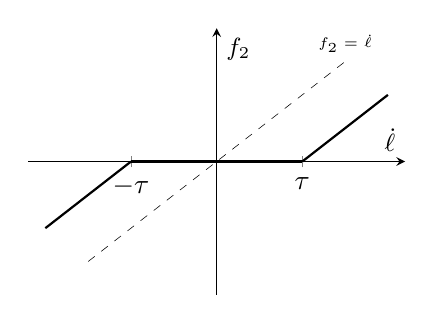
\begin{tikzpicture}
\begin{axis}
[
width = 5cm,
height = 4cm,
scale = 1.4, 
xtick = {-1,0,1}, 
xticklabels = {$-\tau$,0,$\tau$}, 
ytick = {0}, 
ylabel = {\small $f_2$}, 
xlabel = {\small $\dot \ell$}, 
axis x line=middle, 
axis y line=middle,
xmin = -2.2, xmax = 2.2,
ymin = -2, ymax = 2,
every axis plot/.append style={thick}] 
  \addplot[domain=-1:1, samples=10] {0};
  \addplot[domain=1:2, samples=100] {x-1};
  \addplot[domain=-2:-1, samples=100] {x+1};
  \addplot[domain=-1.5:1.5, samples=100, style={very thin,dashed}] {x} node[above] {\tiny$f_2 =\dot \ell$};
\end{axis}
\end{tikzpicture}
\null \vfill
\[
f_2(\dot \ell \, ; \tau) = \left\{\begin{array}{cc}
0 & |\dot \ell| < \tau \\ 
\mathrm{\textbf{sign}}(\dot \ell)(|\dot \ell| - \tau) & |\dot \ell| > \tau \\ 
\end{array}
\right.\] 

\end{multicols}
\end{center}
To set bounds on the altutude, we set $\tau = e_{\mathrm{tol}} k_v k_h$, where $e_{\mathrm{tol}}$ is the allowable distance from the altitude command.
\end{frame}

\begin{frame}
\frametitle{Controller Block Diagram}
\resizebox{11cm}{!}{
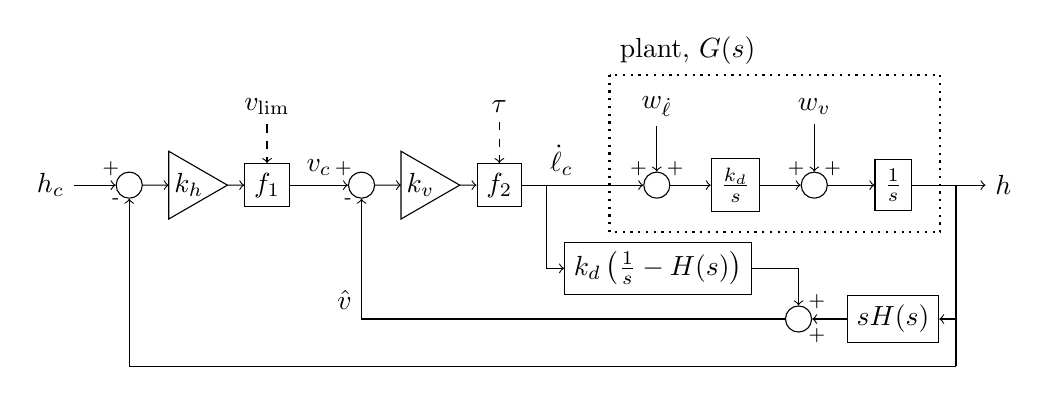
\begin{tikzpicture}[scale=2,
     block/.style = {draw, rectangle,node distance=1cm},
     input/.style = {node distance=1cm},
     output/.style = {node distance=1cm},
     arrow/.style={draw, -latex,node distance=2cm},
     pinstyle/.style = {pin edge={latex-, black,node distance=2cm}},
     sum/.style = {draw, circle, node distance=1cm},
     gain/.style = {regular polygon, regular polygon sides=3,draw, fill=white, text width=1em,
      inner sep=0mm, outer sep=0mm,
      shape border rotate=-90}
    ]
        
    \node [input] (hcmd) {$h_c$};
    \node [sum,right of=hcmd] (hsum) {};    
    \node [gain,right of=hsum, node distance=0.75cm] (K1) {$k_h$};
    \node [block, right of=K1] (N1) {$f_1$};
    \node [sum,right of=N1, node distance=1.2cm] (vsum) {};
    \node [input,above of=N1] (vlim) {$v_{\mathrm{lim}}$};
    \node [gain, right of=vsum,node distance=0.75cm] (K2) {$k_v$};
    \node [block, right of=K2] (N2) {$f_2$};
    \node [sum, right of=N2, node distance=2cm] (dlift) {};
    \node [input,above of=N2] (etol) {$\tau$};
    \node [input, above of=dlift] (ldist) {$w_{\dot \ell}$};
    \node [block, right of=dlift] (lint) {$\frac{k_d}{s}$};
    \node [sum, right of=lint] (velocity) {};
    \node [input, above of=velocity] (vdist) {$w_v$};
    \node [block, right of=velocity] (vint) {$\frac{1}{s}$};
    \node [output, right of=vint,node distance=1.4cm] (h) {$h$};
    \node [block, below of=vint,node distance=1.7cm] (H1) {$sH(s)$};
    \node [block, below right = .6 cm and -1.3 cm of dlift] (H2) {$k_d\left(\frac{1}{s}-H(s)\right)$};
    \node [sum, left of=H1,node distance=1.2cm] (fsum) {};

    \draw[->] (hcmd) -- (hsum) node [above left] {\scriptsize +};
    \draw[->] (hsum) -- (K1);
    \draw[->] (K1) -- (N1);
    \draw[->] (N1) -- node [above] {$v_c$} (vsum) node [above left] {\scriptsize +};
    \draw[->] (vsum) -- (K2);
    \draw[->] (K2) -- (N2);
    \draw[->,dashed] (etol) -- (N2);
    \draw[->,dashed] (vlim) -- (N1);
    \draw[->] (N2) -- node [above left] {$\dot \ell_c$} (dlift)  node [above left] {\scriptsize +};
    \draw[->] (ldist) -- (dlift) node [above right] {\scriptsize +};
    \draw[->] (dlift) -- (lint);
    \draw[->] (lint) -- (velocity) node [above left] {\scriptsize +};
    \draw[->] (vdist) -- (velocity) node [above right] {\scriptsize +};
    \draw[->] (velocity) -- (vint) node [above right] {};
    \draw[->] (vint) -- (h) node [above right] {};
    \draw  (h) ++ (-.3,0) -- ++(0,-1.15) coordinate (fb);
    \draw[->]  (h) ++ (-.3,0) |- (H1);
    \draw[->] (K2) ++ (0.8,0) |- (H2);
    \draw[->] (H1) -- (fsum) node [below right] {\scriptsize +};
    \draw[->] (H2) -| (fsum) node [above right] {\scriptsize +}; 
    \draw[->] (fsum) -| node [above left] {$\hat v$} (vsum) node [below left] {\scriptsize -};
    \draw[->] (fb) -| (hsum) node [below left] {\scriptsize -};
    \draw[thick,dotted] ($(dlift)+(-.3cm,.7cm)$) node [above right] {plant, $G(s)$} rectangle ($(vint)+(.3cm,-.3cm)$) ;
\end{tikzpicture}
}
\resizebox{11cm}{!}{
\begin{tabular}{r l}
$H(s)$ &low-pass filter\\
$f_1(v\,;v_{\mathrm{lim}})$ & clamp on the velocity commanded by the altitude loop set by $v_{\mathrm{lim}}$ \\ 
$f_2(\dot \ell \, ; \tau)$ & deadband on the controller effort set by $\tau$ \\
$h_c$ & commanded altitude \footnotesize (set by Flight Controller) \\
$v_c$ & commanded velocity \footnotesize (output of position loop) \\
$\dot \ell_c$ & commanded change in lift per unit time  \footnotesize (output of velocity loop)\\
$w_{\dot \ell}$ & atmospheric disturbances that change balloon lift  \footnotesize (heating/cooling)\\
$w_v$ & atmospheric disturbances that change balloon velocity \footnotesize (turbulence)\\
$h$ & balloon altitude\\
$\hat v$ & estimate of velocity\\
\end{tabular}
}
\end{frame}

\begin{frame}{Atmosphere Waves}
\begin{center}
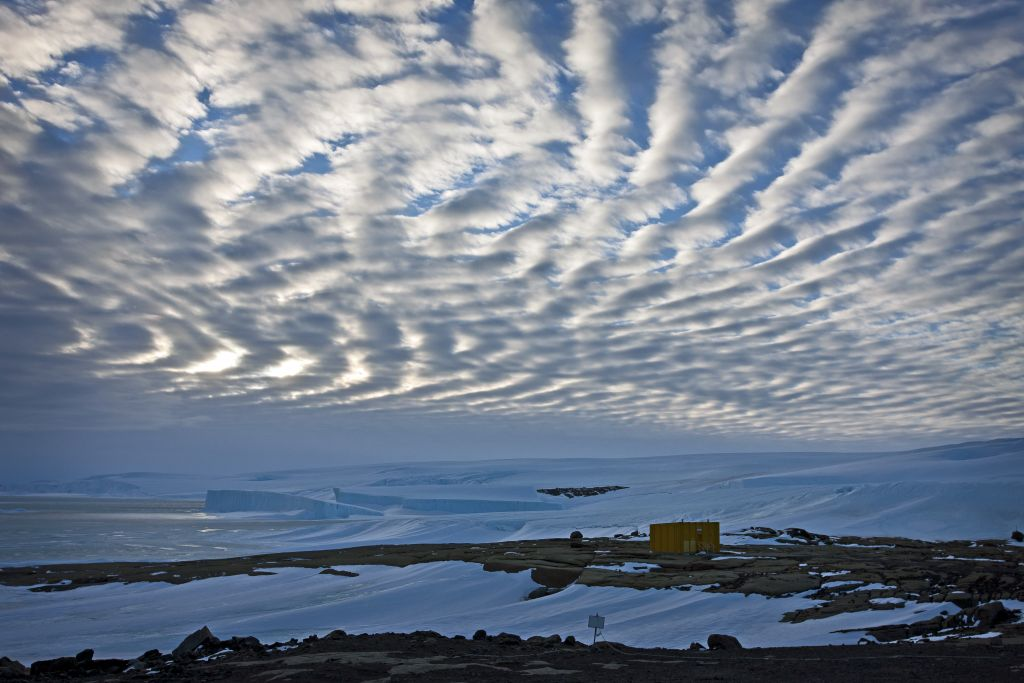
\includegraphics[width=.8\linewidth,trim={0 8cm 0 0cm},clip]{waves.jpg}
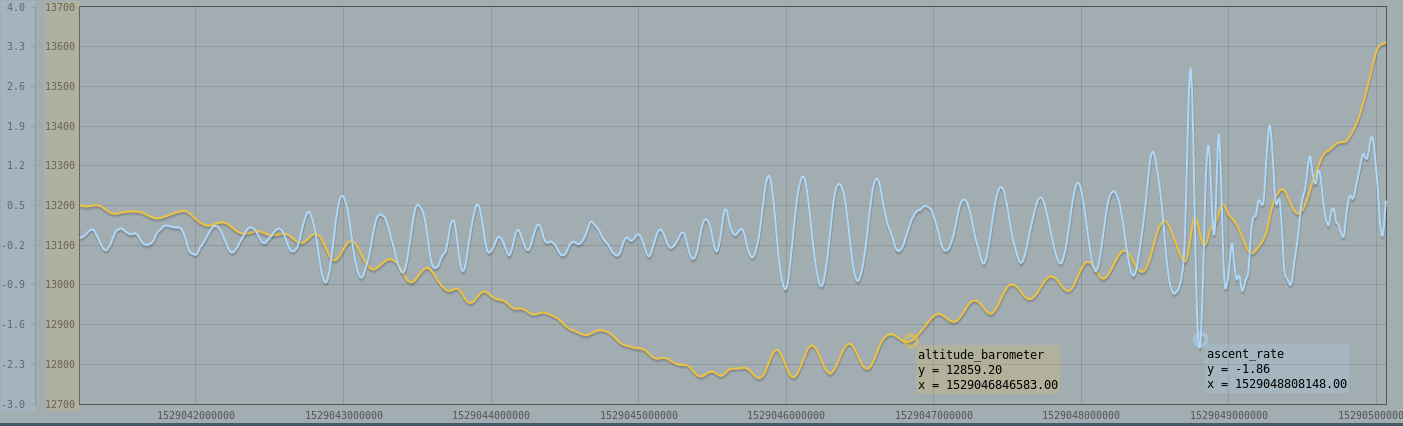
\includegraphics[width=.8\linewidth]{borgwaves.png}
\end{center}
\end{frame}

\begin{frame}{Velocity Estimator}
Low pass filtered velocity estimate uses a 2nd order filter to remove the effect of atmospheric waves
\begin{center}
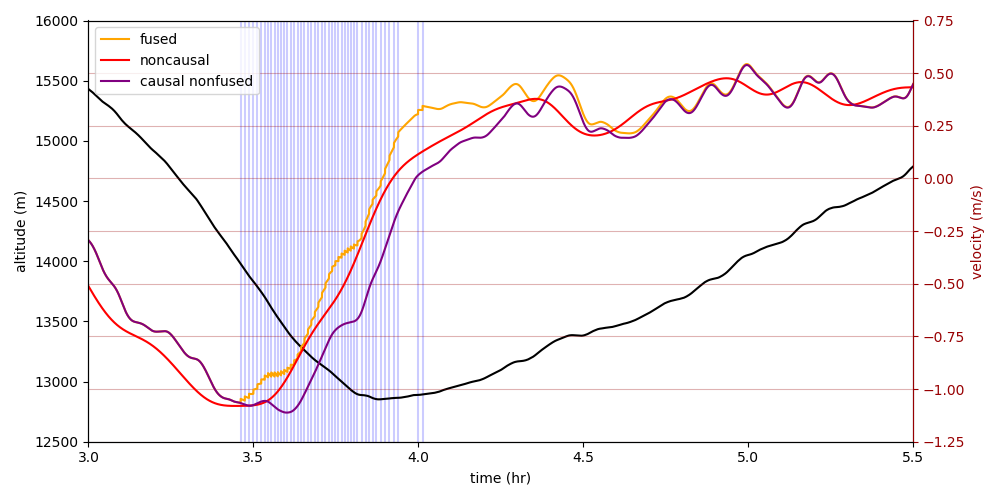
\includegraphics[width=.8\linewidth,trim={10 0 10 0cm},clip]{est.png}
\end{center}
\vspace{-0.5cm}
\[ \mathcal{L}\{ \hat v \} = s H(s) \mathcal{L}\{h\} + \left(\frac{1}{s} - H(s) \right) \mathcal{L} \{\dot l_c\} \]
$H(s)$ a 2nd order lowpass filter\\
\end{frame}

\begin{frame}
\frametitle{Controller Block Diagram}
\resizebox{11cm}{!}{
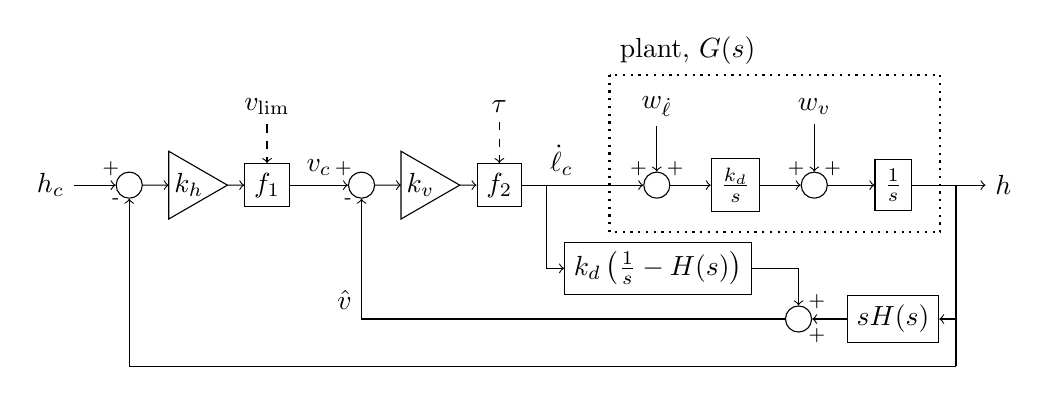
\begin{tikzpicture}[scale=2,
     block/.style = {draw, rectangle,node distance=1cm},
     input/.style = {node distance=1cm},
     output/.style = {node distance=1cm},
     arrow/.style={draw, -latex,node distance=2cm},
     pinstyle/.style = {pin edge={latex-, black,node distance=2cm}},
     sum/.style = {draw, circle, node distance=1cm},
     gain/.style = {regular polygon, regular polygon sides=3,draw, fill=white, text width=1em,
      inner sep=0mm, outer sep=0mm,
      shape border rotate=-90}
    ]
        
    \node [input] (hcmd) {$h_c$};
    \node [sum,right of=hcmd] (hsum) {};    
    \node [gain,right of=hsum, node distance=0.75cm] (K1) {$k_h$};
    \node [block, right of=K1] (N1) {$f_1$};
    \node [sum,right of=N1, node distance=1.2cm] (vsum) {};
    \node [input,above of=N1] (vlim) {$v_{\mathrm{lim}}$};
    \node [gain, right of=vsum,node distance=0.75cm] (K2) {$k_v$};
    \node [block, right of=K2] (N2) {$f_2$};
    \node [sum, right of=N2, node distance=2cm] (dlift) {};
    \node [input,above of=N2] (etol) {$\tau$};
    \node [input, above of=dlift] (ldist) {$w_{\dot \ell}$};
    \node [block, right of=dlift] (lint) {$\frac{k_d}{s}$};
    \node [sum, right of=lint] (velocity) {};
    \node [input, above of=velocity] (vdist) {$w_v$};
    \node [block, right of=velocity] (vint) {$\frac{1}{s}$};
    \node [output, right of=vint,node distance=1.4cm] (h) {$h$};
    \node [block, below of=vint,node distance=1.7cm] (H1) {$sH(s)$};
    \node [block, below right = .6 cm and -1.3 cm of dlift] (H2) {$k_d\left(\frac{1}{s}-H(s)\right)$};
    \node [sum, left of=H1,node distance=1.2cm] (fsum) {};

    \draw[->] (hcmd) -- (hsum) node [above left] {\scriptsize +};
    \draw[->] (hsum) -- (K1);
    \draw[->] (K1) -- (N1);
    \draw[->] (N1) -- node [above] {$v_c$} (vsum) node [above left] {\scriptsize +};
    \draw[->] (vsum) -- (K2);
    \draw[->] (K2) -- (N2);
    \draw[->,dashed] (etol) -- (N2);
    \draw[->,dashed] (vlim) -- (N1);
    \draw[->] (N2) -- node [above left] {$\dot \ell_c$} (dlift)  node [above left] {\scriptsize +};
    \draw[->] (ldist) -- (dlift) node [above right] {\scriptsize +};
    \draw[->] (dlift) -- (lint);
    \draw[->] (lint) -- (velocity) node [above left] {\scriptsize +};
    \draw[->] (vdist) -- (velocity) node [above right] {\scriptsize +};
    \draw[->] (velocity) -- (vint) node [above right] {};
    \draw[->] (vint) -- (h) node [above right] {};
    \draw  (h) ++ (-.3,0) -- ++(0,-1.15) coordinate (fb);
    \draw[->]  (h) ++ (-.3,0) |- (H1);
    \draw[->] (K2) ++ (0.8,0) |- (H2);
    \draw[->] (H1) -- (fsum) node [below right] {\scriptsize +};
    \draw[->] (H2) -| (fsum) node [above right] {\scriptsize +}; 
    \draw[->] (fsum) -| node [above left] {$\hat v$} (vsum) node [below left] {\scriptsize -};
    \draw[->] (fb) -| (hsum) node [below left] {\scriptsize -};
    \draw[thick,dotted] ($(dlift)+(-.3cm,.7cm)$) node [above right] {plant, $G(s)$} rectangle ($(vint)+(.3cm,-.3cm)$) ;
\end{tikzpicture}
}
\resizebox{11cm}{!}{
\begin{tabular}{r l}
$H(s)$ &low-pass filter\\
$f_1(v\,;v_{\mathrm{lim}})$ & clamp on the velocity commanded by the altitude loop set by $v_{\mathrm{lim}}$ \\ 
$f_2(\dot \ell \, ; \tau)$ & deadband on the controller effort set by $\tau$ \\
$h_c$ & commanded altitude \footnotesize (set by Flight Controller) \\
$v_c$ & commanded velocity \footnotesize (output of position loop) \\
$\dot \ell_c$ & commanded change in lift per unit time  \footnotesize (output of velocity loop)\\
$w_{\dot \ell}$ & atmospheric disturbances that change balloon lift  \footnotesize (heating/cooling)\\
$w_v$ & atmospheric disturbances that change balloon velocity \footnotesize (turbulence)\\
$h$ & balloon altitude\\
$\hat v$ & estimate of velocity\\
\end{tabular}
}
\end{frame}

\begin{frame}{Picking gains}
\emph{note:} while the deadband makes the controller non-linear, it still peicewise linear, thus linear analysis can be used.\\
Transfer function for the linear system is\\
\[T(s) = \frac{k_h k_v k_d}{s^2 + k_v k_d s + k_h k_v k_d}.\]
So damping ratio is $\zeta = \frac{1}{2}\sqrt{\frac{k_d k_v}{k_h}}$. 
\begin{itemize}
\item We choose gains such that $\zeta > 1$ and we have over damping.
\item This gives ratio between $k_v$ and $k_h$, but what about magnitiude?
\item high gain $\to$ controller waits and acts agressively near $e_{\n{tol}}$
\item low gain $\to$ controller acts cautiously before $e_{\n{tol}}$
\end{itemize}
demonstraited on next slide
\end{frame}

\begin{frame}{High vs Low Gain}
Plots of simulation shown\\
high gain
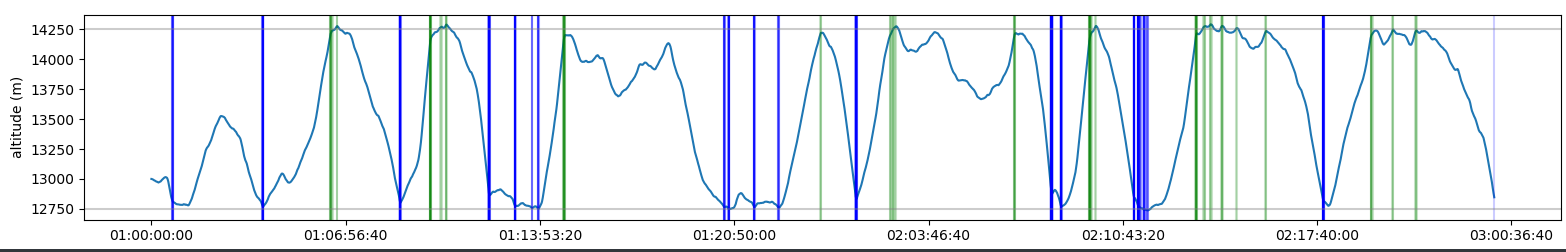
\includegraphics[width=\linewidth,trim={0 5 0 0cm},clip]{highgainsim.png}
\vspace{.05cm}\\
low gain
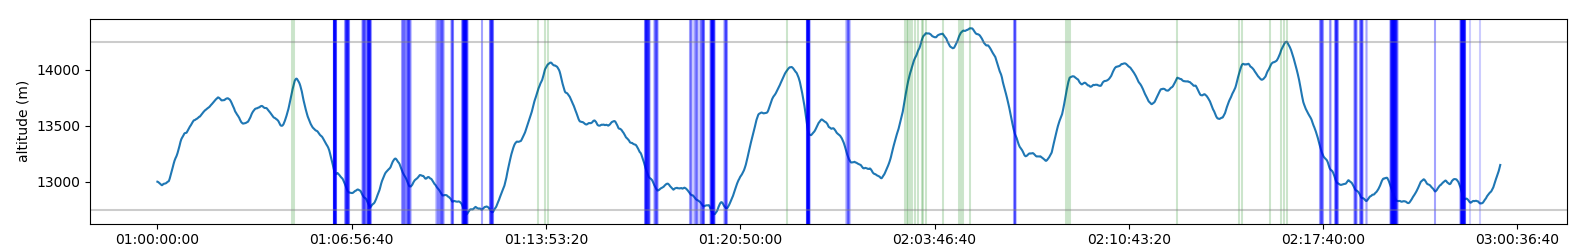
\includegraphics[width=\linewidth,trim={0 0 0 0cm},clip]{lowgainsim.png}

High gain performs better but can't tolerate uncertainty, low gain is worse but performs better under uncertainty
\end{frame}

\begin{frame}{Simulations}
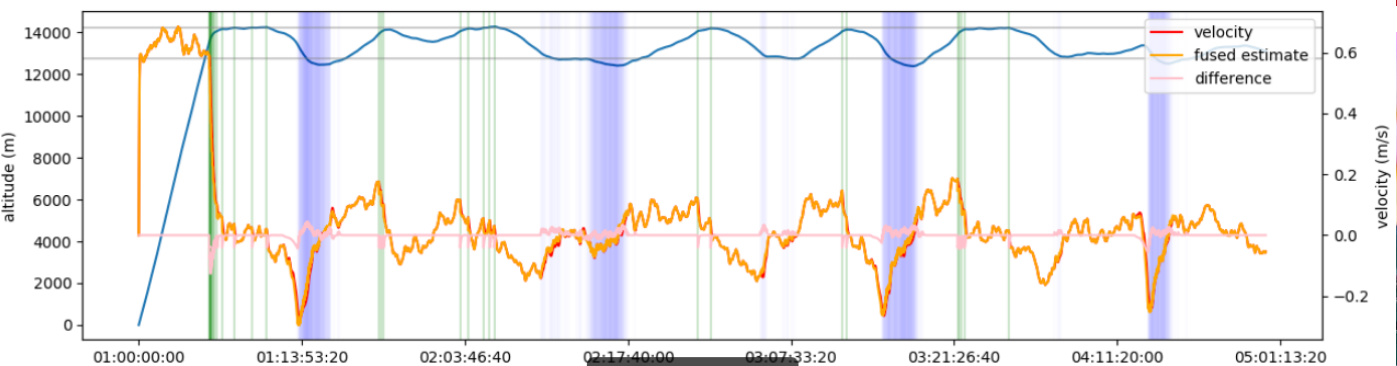
\includegraphics[width=1\linewidth]{lsim.png}
\end{frame}

\begin{frame}{Nightfall}
\begin{columns}
\column{0.55\textwidth}
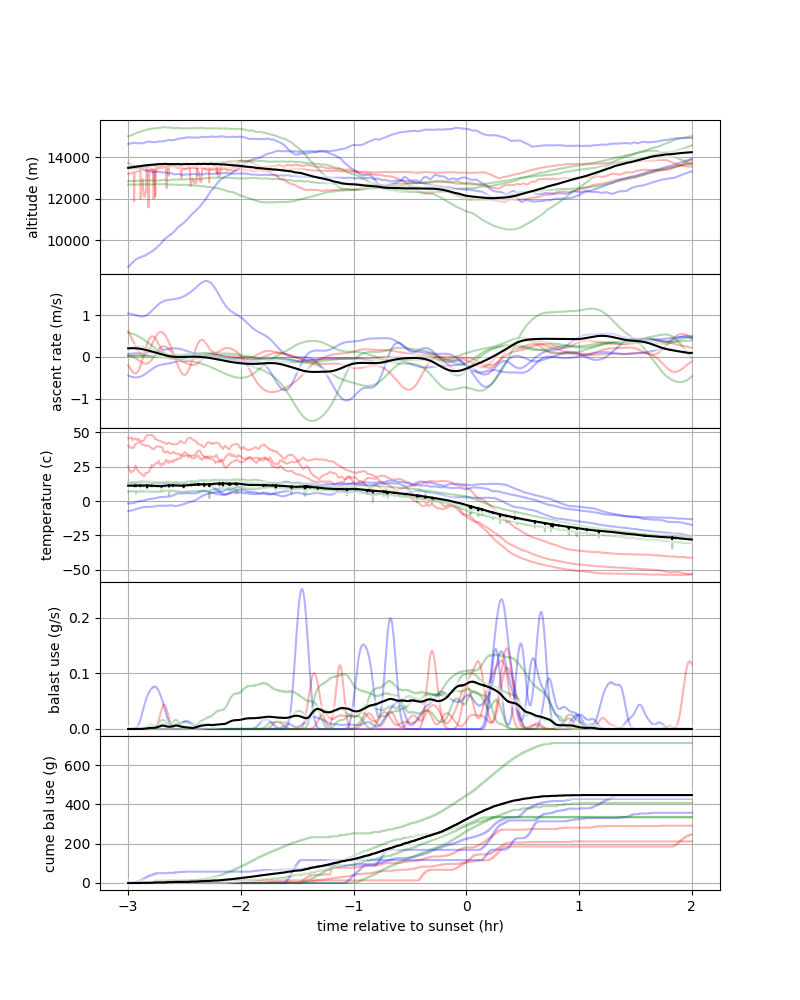
\includegraphics[width=\linewidth,trim={.7cm 0 1cm 3cm},clip]{nightfall_plts.png}
\column{0.55\textwidth}
\begin{itemize}
\item Left plot shows 10 sunsets across various flights (each flight different color).
\item plot blow shows a fit to the data using convex regularization and contraints
\end{itemize}
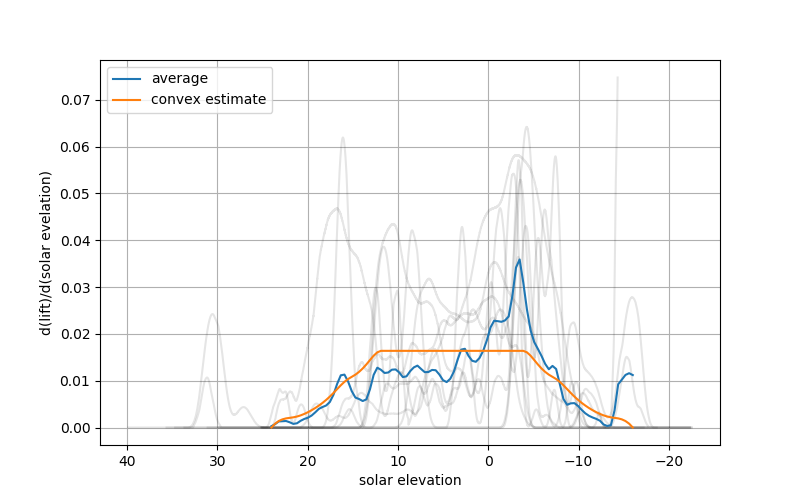
\includegraphics[width=\linewidth,trim={.7cm 0 1cm 1cm},clip]{bal_avg.png}
\end{columns}
\end{frame}


\section{Conclusion}
\begin{frame}{Future Work}
\begin{itemize}\itemsep=24pt
\item Benchmarks
\item Comparison with MCTS
\item 
\end{itemize}
\end{frame}


\end{document}
